%%%%%%%%%%%%%%%%%%%%%%%%%%%%%%%%%%%%%%%%%%%%%%%%%%
%% Allgemeiner Header mit scrreprt				%%
%% Autor: Stefan Zollinger						%%
%% Quellen:	-scrguide							%%		
%%			-www.dante.de						%%
%%%%%%%%%%%%%%%%%%%%%%%%%%%%%%%%%%%%%%%%%%%%%%%%%%

%-------------------------------------------------
%Dokumentklasse und allgemeine Pakete
%-------------------------------------------------
\documentclass[
		11pt, 
		bibliography=totocnumbered,		    %Literaturverzeichnis im Inhaltsverzeichnis 
	  listof=totocnumbered,							%Tab. und Abb.-verzeichnis nummeriert	
		final,												%f�r endversion (draft -> ohne bilder und links, 
		                              %anzeige von Fehlern)
		parskip=half,									%Halbe Zeile Abstand zwischen Abs�tzen.
		twoside=false									%zweiseitig
		]{scrreprt} 	

\usepackage{scrhack}					%beseitigt warnung wegen float+koma inkompatibilit�t
\usepackage[T1]{fontenc}			%umlaute als eigene Zeichen
\usepackage[latin1]{inputenc}	%umlaute erkennen
\usepackage[ngerman]{babel}		%silbentrennung englische Rechtschreibung
\usepackage{babelbib}					%f�r deutsches literaturverzeichnis
%\usepackage{scrpage2}					%pagestyle
\usepackage{lastpage}					%f�r Referenzen auf letzte Seite
\usepackage{textcomp}					%einige Sonderzeichen
\usepackage{graphicx}	        %grafiken in jpeg,png
\usepackage{epstopdf}		    	%f�r .eps vektorgrafiken
\usepackage{color}						%ben�tigt f�r farbeinstellungen
\usepackage{array}				    %erweiterte Optionen in tabellen (Bsp. ausrichtung innerhalb felder)
\usepackage{subfigure}				%um 2 bilder nebeneinander anzuzeigen
\usepackage{amsmath} 					%mathematischen Textsatz.
\usepackage{amssymb}					%	-Erweiterte math. Sonderzeichen
\usepackage{dsfont}						%	-Mengen			
\usepackage{paralist} 				%kompakte Aufz�hlung: \begin{compactitem}
\usepackage{float}						%f�r H option bei floats(figure,table)
\usepackage{lmodern}					%moderne Schrift
\usepackage{url}				   	 	%korrekte darstellung von urls (mit verlinkung)
\usepackage{changepage}       %f�r adjustwidth auf titelseite
\usepackage{fancyhdr}					%f�r \pagestyle{fancy} -> kopf/fusszeile �ber Textk�rper hinaus
\usepackage{acronym}					%abk�rzungsverzeichnis, Anwendung: \ac{KDE}
\usepackage{cellspace}				%f�r S-operator in Tabellen -> Formeln ber�hren R�nder nicht
\usepackage{booktabs}					%Tabellen: \toprule \midrule \bottomrule
\usepackage{mparhack}         %Repariert falsch gesetzte marginalien am Seitenanfang
\usepackage{setspace}
\usepackage{placeins}

%-------------------------------------------------
% formatierte Listings
%-------------------------------------------------	
\definecolor{commentColor}{rgb}{0.3,0.3,0.3}	%Grau f�r kommentare in Listings
\usepackage{listings}
\lstset{ %
language=Matlab,                % choose the language of the code
basicstyle=\small \ttfamily,    % font style
numbers=none,                   % where to put the line-numbers
numberstyle=\small \ttfamily,      % the size of the fonts that are used for the line-numbers
commentstyle=\color{commentColor},				%kommentare
stepnumber=1,                   % the step between two line-numbers. If it's 1 each line will be numbered
numbersep=5pt,                  % how far the line-numbers are from the code�
xleftmargin=15pt,               % linker rand
xrightmargin=15pt,               % rechter rand
backgroundcolor=\color{white},  % choose the background color. requires \usepackage{color}
showspaces=false,               % show spaces adding particular underscores
showstringspaces=false,         % underline spaces within strings
showtabs=false,                 % show tabs within strings adding particular underscores
frame=lines,  	                  % frame: none|leftline|topline|bottomline|lines|single|shadowboxi
tabsize=2,	                    % sets default tabsize to 2 spaces
captionpos=t,                   % sets the caption-position t/b
breaklines=true,                % sets automatic line breaking
breakatwhitespace=false,        % sets if automatic breaks should only happen at whitespace
escapeinside={\%*}{*)}          % if you want to add a comment within your code
}


%-------------------------------------------------
% Abk�rzungsverzeichnis implementieren
%-------------------------------------------------									
\usepackage{nomencl} 				
\renewcommand{\nomname}{List of abbreviations}
\makenomenclature					%abk.verz. umbenennen

%kommando zum einfachen einstellen der Schrift
% Bsp. \changefont{lmss}{sbc}{n}  %latin modern bold condensed Schriftart der Titel
%      \changefont{lmss}{m}{n}		%latin modern sans serif
\newcommand{\changefont}[3]{\fontfamily{#1}\fontseries{#2}\fontshape{#3}\selectfont}
  
%-------------------------------------------------
% Marginalien/Seitenr�nder
%-------------------------------------------------
\newcommand{\marg}[1]{\marginpar{\raggedright \changefont{lmss}{m}{n} #1}}	
%marginalien linksb�ndig mit \marg{text der marginalie}

%\usepackage[
%			%includemp,				%marginalien in Textk�rper einbeziehen
%			%includeall,
%			%showframe,				%zeigt rahmen zum debuggen		
%			marginparwidth=30mm, 	%breite der marginalien
%			marginparsep=5mm,		%abstand marginalien - text
%			reversemarginpar,		%marginalien links statt rechts
%			left=45mm,				%abstand von Seitenraendern
%			right=25mm,				%
%			top=30mm,
%			bottom=30mm,
%			twoside
%			]{geometry}
			
\usepackage[
			%includemp,				%marginalien in Textk�rper einbeziehen
			%includeall,
			%showframe,				%zeigt rahmen zum debuggen		
			marginparwidth=30mm, 	%breite der marginalien
			marginparsep=5mm,		%abstand marginalien - text
			%reversemarginpar,		%marginalien links statt rechts
			left=25mm,				%abstand von Seitenraendern
			right=45mm,				%
			top=20mm,
			bottom=20mm,
			oneside
			]{geometry}
			
%-------------------------------------------------
%Kopf-/Fusszeile
%-------------------------------------------------
%\pagestyle{scrheadings}
%\clearscrheadfoot															%voreinstellungen l�schen
%\automark[chapter]{chapter}										%Kapitelangabe 
%\ihead{\changefont{lmss}{sbc}{n} \headmark}		%kopfzeile
%\ifoot[																				%fusszeile
%        \changefont{lmss}{m}{n}{ \thepage  /\pageref{LastPage}}]
%        {\changefont{lmss}{m}{n}{ \thepage  /\pageref{LastPage}}}	
        
        
        
%%% Kopf und Fusszeilen
\pagestyle{fancy}					%stil der kopf/fusszeilen 
\renewcommand{\chaptermark}[1]{\markboth{\thechapter.\ #1}{}}	
%damit Kapitelangaben im Header kleingeschrieben werden
\fancyhead{} 						% clear all header fields
\fancyhead[RE,LO]{ \changefont{lmss}{sbc}{n} \leftmark }
\fancyhead[C]{ }
\fancyhead[LE,RO]{ \changefont{lmss}{m}{n} \thepage/\pageref{LastPage} }
%\fancyhead[LO]{\changefont{lmss}{m}{n} \thepage/\pageref{LastPage} \hspace{2.5cm}
%							 \changefont{lmss}{sbc}{n} \leftmark }
\fancyfoot{} 						% clear all footer fields
\fancyfoot[LE,RO]{ }
\fancyfoot[C]{}
\fancyfoot[RE,LO]{  }
\renewcommand{\headrulewidth}{0.5pt}
\renewcommand{\footrulewidth}{0pt}
\fancyhfoffset[LE,RO]{35mm} 			%header und footer nach links verlängern (über marginalien)
\fancypagestyle{plain}{				% plain redefinieren, damit wirklich alle seiten im gleichen stil sind (ausser titlepage)
	\pagestyle{fancy}
}

%-------------------------------------------------
%PDF-Optionen
%-------------------------------------------------
\usepackage[%
	pdftitle={SA},%                                   Titel des PDF Dokuments.
	pdfauthor={Autoren},%                                Autor des PDF Dokuments.
	pdfsubject={Thema},%                                 Thema des PDF Dokuments.
	pdfcreator={LaTeX with hyperref and KOMA-Script},%   Erzeuger des PDF Dokuments.
	pdfkeywords={Schuelsselwrter},%                        auch fr PDF Dokumente indexiert.)
	pdfpagemode=UseOutlines,%                            Inhaltsverzeichnis anzeigen beim ffnen
	pdfdisplaydoctitle=false,%                            Dokumenttitel statt Dateiname anzeigen.
	pdflang=de%                                          Sprache des Dokuments.
]{hyperref}

\definecolor{LinkColor}{rgb}{0,0,0}	%{0,0,0.4} -> Blaue Links im PDF Dokument.
\hypersetup{%
	colorlinks=true,%        Aktivieren von farbigen Links im Dokument (keine Rahmen)
	linkcolor=LinkColor,%    Farbe festlegen.
	citecolor=LinkColor,%    Farbe festlegen.
	filecolor=LinkColor,%    Farbe festlegen.
	menucolor=LinkColor,%    Farbe festlegen.
	urlcolor=LinkColor,%     Farbe von URL's im Dokument.
	bookmarksnumbered=true%  berschriftsnummerierung im PDF Inhalt anzeigen.
}

% bessere float plazierung
\renewcommand{\textfraction}{0.1}
\renewcommand{\topfraction}{0.9}
\renewcommand{\bottomfraction}{0.9}
\renewcommand{\floatpagefraction}{0.35}
\setcounter{totalnumber}{5}

\let\origsection\section								%\section sichern als \origsection
\renewcommand{\section}{\FloatBarrier \origsection}		%\section �berschreiben 
														%\FloatBarrier: verhindert, dass Bilder oder Tab. hier weiterrutschen


\begin{document}
\pagestyle{fancy}
%\lhead{Optimierung}
\frontmatter
\newcommand\HRule{\noindent\rule{\linewidth}{1.5pt}}

\begin{titlepage}
\vspace*{\stretch{1}}
\HRule
\vspace*{10pt}
\begin{flushright}
{\Huge
Simplex Algorithmus f"ur nichtlineare Optimierungsprobleme}
\end{flushright}
\HRule
\begin{flushright}
\vspace{30pt}
\LARGE
Selina Malacarne, Raphael Nestler
\end{flushright}
\vspace*{\stretch{2}}
\begin{center}
Hochschule f"ur Technik, Rapperswil, 2012
\end{center}
\end{titlepage}

\hypersetup{
    colorlinks=true,
    linktoc=all,
    linkcolor=blue
}

\setcounter{tocdepth}{2}
\tableofcontents
\mainmatter

\section{Einleitung}
Der Simplex-Downhill-Algorithmus ist eine Methode zur Optimierung nichtlinearer n-dimensionaler Funktionen.

Dieses Verfahren wurde von den britischen Statistikern John Nelder und Roger Mead entwickelt und gilt vor allem bei Problemen mit geringem rechnerischen Aufwand als die schnellstm"ogliche Methode.
Ein  klarer Vorteil dieser Methode ist, dass sie auf Probleme angewendet werden kann, bei denen  die Ableitungen nicht bekannt sind oder gar nicht existieren.
Die Methode kann hilfreich sein, um (sinnvolle) Versuchspunkte zu ermitteln, welche dann in eine Simulation eingespeist werden.
Dies hat den Vorteil, dass eine teure (sprich zeit- und rechenaufwendig) Simulation nicht einfach sinnlose Datenmengen rechnet, die man schlussendlich verwerfen muss, weil sie physikalisch keinen Sinn ergeben.


%\chapter{Simplex-Downhill}
%--------------------------------------------------------------------------------------------------------------------------------------------
%General Stuff
%--------------------------------------------------------------------------------------------------------------------------------------------
\section{Simplex}
Das Simplex ist ein Begriff, welcher aus der Geometrie stammt. Es beschreibt ein n-dimensionales Polytop. Wobei ein Polytop die Bezeichnung für ein verallgemeinertes Polygon ist, sprich ein verallgemeinertes Vieleck. 
Hier einige vorstellbare Beispiele zum Simplex:\\
 
\begin{tabular}{c|l}
Dimension & Geometrische Form\\
\hline
$n=0$ & Punkt\\
$n=1$ & Strecke\\
$n=2$ & Dreieck\\
$n=3$ & Tetraeder
\end{tabular} 

Aus der Tabelle wird ersichtlich, dass jedes n-dimensionale Simplex genau n+1 Ecken hat.
Im Downhill-Simplex-Verfahren wird das Simplex benötigt, um die optimalen Parameterwerte zu finden. Man kann es sich so vorstellen, dass das Simplex im n-dimensionalen Parameterraum aufgespannt wird und dann für jeden seiner Eckpunkte den entsprechenden Funktionswert (auf Grund der Zielfunktion) berechnet. \\
Wie in der Einleitung schon erwähnt worden ist, arbeitet der Simplex-Downhill Algorithmus ohne Ableitungen. Warum das funktioniert wird klar, wenn man sich vorstellt, dass das Simplex selber auf der Zielfunktion liegt und sozusagen die Ableitung imitiert. Sucht der Algorithmus ein Minimum, so bewegt er sich natürlich abwärts (downhill), was auch seine Namensgebung erklärt. Der Algorithmus ist aber ebenfalls in der Lage nach Maxima zu suchen, wobei im Folgenden nur die Suche nach Minima behandelt wird.\\
Hat man das Simplex auf der Zielfunktion platziert, werden die berechneten Testpunkte geprüft, wobei der schlechteste dieser Punkte dann mittels gewisser "Taktiken" ersetzt wird. Dies wird solange fort geführt, bis das gewünschte Ergebnis erreicht worden ist.\\ 
Im nächsten Abschnitt werden die möglichen Taktiken, um das Simplex zu verändern, genauer erläutert. 

%--------------------------------------------------------------------------------------------------------------------------------------------

\section{Modifikationen des Simplex}
Die Möglichkeiten das Simplex soweit zu verändern, dass es den optimalen Punkt findet, sind begrenzt.
Die Darstellungen beziehen sich hierbei auf einen Simplex der zweiten Dimension (Dreieck), natürlich gelten diese Modifikationen auch für einen n-dimensionalen Simplex. Der Algorithmus wählt auf Grund der Werte der Eckpunkte beziehungsweise deren Zielfunktionswerte die Modifikationsart aus (siehe Kapitel XXX).

\begin{figure}[h]
	\centering
	\definecolor{uuuuuu}{rgb}{0.27,0.27,0.27}
\definecolor{zzttqq}{rgb}{0.6,0.2,0}
\definecolor{qqqqff}{rgb}{0,0,1}
\begin{tikzpicture}[line cap=round,line join=round,>=triangle 45,x=1.0cm,y=1.0cm]
\clip(5.32,0.26) rectangle (11.46,4.08);
\fill[color=zzttqq,fill=zzttqq,fill opacity=0.1] (5.74,2.92) -- (10.36,3.74) -- (11,1.52) -- cycle;
\draw [color=zzttqq] (5.74,2.92)-- (10.36,3.74);
\draw [color=zzttqq] (10.36,3.74)-- (11,1.52);
\draw [color=zzttqq] (11,1.52)-- (5.74,2.92);
\draw [color=zzttqq] (11,1.52)-- (5.74,2.92);
\begin{scriptsize}
\fill [color=qqqqff] (5.74,2.92) circle (1.5pt);
\draw[color=qqqqff] (5.75,3.02) node {$x_{min}$};
\fill [color=qqqqff] (10.36,3.74) circle (1.5pt);
\draw[color=qqqqff] (10.51,3.81) node {$x_{max}$};
\fill [color=qqqqff] (11,1.52) circle (1.5pt);
\draw[color=qqqqff] (11.07,1.59) node {$x_3$};
\fill [color=uuuuuu] (9.03,2.73) circle (1.5pt);
\draw[color=uuuuuu] (9.13,2.7) node {$x_m$};
\end{scriptsize}
\end{tikzpicture}
%
  	\caption{Simplex im zweidimensionalen Raum}%
	\label{fig:Dreieck}%
\end{figure}

\subsection{Reflexion}
Bei der Reflexion wird der schlechteste Punkt $x_{max}$ am Schwerpunkt des Simplex gespiegelt und mit einem Faktor $\alpha$ gewichtet: 
\begin{equation}
x_{ref} = x_m + \alpha \cdot (x_m-x_{max})
\end{equation}
Wenn ein neues Simplex berechnet werden muss, weil der optimale wert noch nicht gefunden worden ist, dann wird die Reflexion IMMER durchgeführt, daher wird in den folgenden Methoden manchmal mit $x_{ref}$ anstatt mit $x_{max}$ gerechnet. Wenn man den Algorithmus unter XXX betrachtet, erkennt man, warum das so ist.  
\begin{figure}[h]
	\centering
	\definecolor{uuuuuu}{rgb}{0.27,0.27,0.27}
\definecolor{zzttqq}{rgb}{0.6,0.2,0}
\definecolor{qqqqff}{rgb}{0,0,1}
\begin{tikzpicture}[line cap=round,line join=round,>=triangle 45,x=1.0cm,y=1.0cm]
\clip(5.32,0.26) rectangle (11.46,4.08);
\fill[color=zzttqq,fill=zzttqq,fill opacity=0.1] (5.74,2.92) -- (10.36,3.74) -- (11,1.52) -- cycle;
\fill[color=zzttqq,fill=zzttqq,fill opacity=0.1] (5.74,2.92) -- (7.71,1.71) -- (11,1.52) -- cycle;
\draw [color=zzttqq] (5.74,2.92)-- (10.36,3.74);
\draw [color=zzttqq] (10.36,3.74)-- (11,1.52);
\draw [color=zzttqq] (11,1.52)-- (5.74,2.92);
\draw (9.03,2.73)-- (7.71,1.71);
\draw [color=zzttqq] (5.74,2.92)-- (7.71,1.71);
\draw [color=zzttqq] (7.71,1.71)-- (11,1.52);
\draw [color=zzttqq] (11,1.52)-- (5.74,2.92);
\draw [color=zzttqq] (11,1.52)-- (5.74,2.92);
\begin{scriptsize}
\fill [color=qqqqff] (5.74,2.92) circle (1.5pt);
\draw[color=qqqqff] (5.75,3.02) node {$x_{min}$};
\fill [color=qqqqff] (10.36,3.74) circle (1.5pt);
\draw[color=qqqqff] (10.51,3.81) node {$x_{max}$};
\fill [color=qqqqff] (11,1.52) circle (1.5pt);
\draw[color=qqqqff] (11.07,1.59) node {$x_3$};
\fill [color=uuuuuu] (9.03,2.73) circle (1.5pt);
\draw[color=uuuuuu] (9.13,2.7) node {$x_m$};
\fill [color=qqqqff] (7.71,1.71) circle (1.5pt);
\draw[color=qqqqff] (7.91,1.67) node {$x_{ref}$};
\end{scriptsize}
\end{tikzpicture}
%
  	\caption{Reflexion}%
	\label{fig:Reflexion}%
\end{figure}

\subsection{Expansion}
Bei der Expansion wird der Schwerpunkt $x_m$ mit dem Faktor $\gamma$ in Richtung $x_{ref}$ gestreckt. 

\begin{equation}
x_{streck} = x_{ref} + \gamma \cdot (x_{ref}-x_{m})
\end{equation}
\begin{figure}[h]
	\centering
	\resizebox{1\textwidth}{!}{
\definecolor{uuuuuu}{rgb}{0.27,0.27,0.27}
\definecolor{zzttqq}{rgb}{0.6,0.2,0}
\definecolor{qqqqff}{rgb}{0,0,1}
\begin{tikzpicture}[line cap=round,line join=round,>=triangle 45,x=1.0cm,y=1.0cm]
\clip(4.51,0.05) rectangle (11.48,4.25);
\fill[color=zzttqq,fill=zzttqq,fill opacity=0.1] (5.74,3) -- (10.36,4) -- (11,2) -- cycle;
\fill[color=zzttqq,fill=zzttqq,fill opacity=0.1] (5.74,3) -- (6.38,1) -- (11,2) -- cycle;
\fill[color=zzttqq,fill=zzttqq,fill opacity=0.1] (5.74,3) -- (5.39,0.25) -- (11,2) -- cycle;
\draw [color=zzttqq] (5.74,3)-- (10.36,4);
\draw [color=zzttqq] (10.36,4)-- (11,2);
\draw [color=zzttqq] (11,2)-- (5.74,3);
\draw (8.37,2.5)-- (6.38,1);
\draw (8.37,2.5)-- (5.39,0.25);
\draw [color=zzttqq] (5.74,3)-- (6.38,1);
\draw [color=zzttqq] (6.38,1)-- (11,2);
\draw [color=zzttqq] (11,2)-- (5.74,3);
\draw [color=zzttqq] (5.74,3)-- (5.39,0.25);
\draw [color=zzttqq] (5.39,0.25)-- (11,2);
\draw [color=zzttqq] (11,2)-- (5.74,3);
\begin{scriptsize}
\fill [color=qqqqff] (5.74,3) circle (1.5pt);
\draw[color=qqqqff] (5.75,3.11) node {$x_{min}$};
\fill [color=qqqqff] (10.36,4) circle (1.5pt);
\draw[color=qqqqff] (10.53,4.07) node {$x_{max}$};
\fill [color=qqqqff] (11,2) circle (1.5pt);
\draw[color=qqqqff] (11.08,2.08) node {$x_3$};
\fill [color=uuuuuu] (8.37,2.5) circle (1.5pt);
\draw[color=uuuuuu] (8.48,2.47) node {$x_m$};
\fill [color=qqqqff] (6.38,1) circle (1.5pt);
\draw[color=qqqqff] (6.62,0.95) node {$x_{ref}$};
\fill [color=uuuuuu] (5.39,0.25) circle (1.5pt);
\draw[color=uuuuuu] (5.6,0.19) node {$x_{streck}$};
\end{scriptsize}
\end{tikzpicture}
}
%
  	\caption{Expansion}%
	\label{fig:Streckung}%
\end{figure}
\newpage
\subsection{Kontraktion 1}
Bei der Kontraktion 1 wird der schlechteste Punkt um den Faktor $\beta$ näher an den Schwerpunkt $x_m$ gerückt. 
\begin{equation}
x_{kon} = x_{m} + \beta \cdot (x_{max}-x_{m})
\end{equation}

\begin{figure}[h]
	\centering
	\resizebox{1\textwidth}{!}{
\definecolor{uuuuuu}{rgb}{0.27,0.27,0.27}
\definecolor{zzttqq}{rgb}{0.6,0.2,0}
\definecolor{qqqqff}{rgb}{0,0,1}
\begin{tikzpicture}[line cap=round,line join=round,>=triangle 45,x=1.0cm,y=1.0cm]
\clip(4.51,0.05) rectangle (11.48,4.25);
\fill[color=zzttqq,fill=zzttqq,fill opacity=0.1] (5.74,3) -- (10.36,4) -- (11,2) -- cycle;
\fill[color=zzttqq,fill=zzttqq,fill opacity=0.1] (5.74,3) -- (9.37,3.25) -- (11,2) -- cycle;
\draw [color=zzttqq] (5.74,3)-- (10.36,4);
\draw [color=zzttqq] (10.36,4)-- (11,2);
\draw [color=zzttqq] (11,2)-- (5.74,3);
\draw [color=zzttqq] (11,2)-- (5.74,3);
\draw [color=zzttqq] (5.74,3)-- (9.37,3.25);
\draw [color=zzttqq] (9.37,3.25)-- (11,2);
\draw [color=zzttqq] (11,2)-- (5.74,3);
\begin{scriptsize}
\fill [color=qqqqff] (5.74,3) circle (1.5pt);
\draw[color=qqqqff] (5.75,3.11) node {$x_{min}$};
\fill [color=qqqqff] (10.36,4) circle (1.5pt);
\draw[color=qqqqff] (10.53,4.07) node {$x_{max}$};
\fill [color=qqqqff] (11,2) circle (1.5pt);
\draw[color=qqqqff] (11.08,2.08) node {$x_3$};
\fill [color=uuuuuu] (8.37,2.5) circle (1.5pt);
\draw[color=uuuuuu] (8.48,2.47) node {$x_m$};
\fill [color=uuuuuu] (9.37,3.25) circle (1.5pt);
\draw[color=uuuuuu] (9.59,3.3) node {$x_{kon}$};
\end{scriptsize}
\end{tikzpicture}
}
%
  	\caption{Kontraktion 1}%
	\label{fig:Kon1}%
\end{figure}

\subsection{Kontraktion 2}
Bei der Kontraktion 2 wird der reflektierte Punkt um den Faktor $\beta$ näher an den Schwerpunkt $x_m$ gerückt. 
\begin{equation}
x_{kon} = x_{m} + \beta \cdot (x_{ref}-x_{m})
\end{equation}

\begin{figure}[h]
	\centering
	\resizebox{1\textwidth}{!}{
\definecolor{uuuuuu}{rgb}{0.27,0.27,0.27}
\definecolor{zzttqq}{rgb}{0.6,0.2,0}
\definecolor{qqqqff}{rgb}{0,0,1}
\begin{tikzpicture}[line cap=round,line join=round,>=triangle 45,x=1.0cm,y=1.0cm]
\clip(4.51,0.05) rectangle (11.48,4.25);
\fill[color=zzttqq,fill=zzttqq,fill opacity=0.1] (5.74,3) -- (10.36,4) -- (11,2) -- cycle;
\fill[color=zzttqq,fill=zzttqq,fill opacity=0.1] (5.74,3) -- (6.38,1) -- (11,2) -- cycle;
\fill[color=zzttqq,fill=zzttqq,fill opacity=0.1] (5.74,3) -- (7.38,1.75) -- (11,2) -- cycle;
\draw [color=zzttqq] (5.74,3)-- (10.36,4);
\draw [color=zzttqq] (10.36,4)-- (11,2);
\draw [color=zzttqq] (11,2)-- (5.74,3);
\draw (8.37,2.5)-- (6.38,1);
\draw [color=zzttqq] (5.74,3)-- (6.38,1);
\draw [color=zzttqq] (6.38,1)-- (11,2);
\draw [color=zzttqq] (11,2)-- (5.74,3);
\draw [color=zzttqq] (11,2)-- (5.74,3);
\draw [color=zzttqq] (5.74,3)-- (7.38,1.75);
\draw [color=zzttqq] (7.38,1.75)-- (11,2);
\draw [color=zzttqq] (11,2)-- (5.74,3);
\begin{scriptsize}
\fill [color=qqqqff] (5.74,3) circle (1.5pt);
\draw[color=qqqqff] (5.75,3.11) node {$x_{min}$};
\fill [color=qqqqff] (10.36,4) circle (1.5pt);
\draw[color=qqqqff] (10.53,4.07) node {$x_{max}$};
\fill [color=qqqqff] (11,2) circle (1.5pt);
\draw[color=qqqqff] (11.08,2.08) node {$x_3$};
\fill [color=uuuuuu] (8.37,2.5) circle (1.5pt);
\draw[color=uuuuuu] (8.48,2.47) node {$x_m$};
\fill [color=qqqqff] (6.38,1) circle (1.5pt);
\draw[color=qqqqff] (6.62,0.95) node {$x_{ref}$};
\fill [color=uuuuuu] (7.38,1.75) circle (1.5pt);
\draw[color=uuuuuu] (7.58,1.7) node {$x_{kon2}$};
\end{scriptsize}
\end{tikzpicture}
}
%
  	\caption{Kontraktion 2}%
	\label{fig:Kon2}%
\end{figure}
\newpage
\subsection{Komprimierung}
Die Komprimierung ist die letzte Modifikation und ist sozusagen die '"letzte Hoffnung"', wenn alles andere vorher nichts gebracht hat. Hierbei werden alle Ecken $x_i$ des Simplex zum besten Punkt $x_{min}$ hingezogen, auch hier kann man diese Zusammenziehung mit dem Faktor $\beta$ steuern.  
\begin{equation}
x_{i} = (x_i + x_{min}) \cdot \beta
\end{equation}

\begin{figure}[h]
	\centering
	\resizebox{0.8\textwidth}{!}{
\definecolor{uuuuuu}{rgb}{0.27,0.27,0.27}
\definecolor{zzttqq}{rgb}{0.6,0.2,0}
\definecolor{qqqqff}{rgb}{0,0,1}
\begin{tikzpicture}[line cap=round,line join=round,>=triangle 45,x=1.0cm,y=1.0cm]
%\clip(4.51,0.05) rectangle (11.48,4.25);
\fill[color=zzttqq,fill=zzttqq,fill opacity=0.1] (5.74,3) -- (10.36,4) -- (11,2) -- cycle;
\fill[color=zzttqq,fill=zzttqq,fill opacity=0.1] (5.74,3) -- (8.05,3.5) -- (8.37,2.5) -- cycle;
\draw [color=zzttqq] (5.74,3)-- (10.36,4);
\draw [color=zzttqq] (10.36,4)-- (11,2);
\draw [color=zzttqq] (11,2)-- (5.74,3);
\draw [color=zzttqq] (11,2)-- (5.74,3);
\draw [color=zzttqq] (5.74,3)-- (8.05,3.5);
\draw [color=zzttqq] (8.05,3.5)-- (8.37,2.5);
\draw [color=zzttqq] (8.37,2.5)-- (5.74,3);
\begin{scriptsize}
\fill [color=qqqqff] (5.74,3) circle (1.5pt);
\draw[color=qqqqff] (5.75,3.11) node {$x_{min}$};
\fill [color=qqqqff] (10.36,4) circle (1.5pt);
\draw[color=qqqqff] (10.53,4.07) node {$x_{max}$};
\fill [color=qqqqff] (11,2) circle (1.5pt);
\draw[color=qqqqff] (11.08,2.08) node {$x_3$};
\fill [color=uuuuuu] (8.37,2.5) circle (1.5pt);
\draw[color=uuuuuu] (8.59,2.61) node {$x_{3neu}$};
\fill [color=uuuuuu] (8.05,3.5) circle (1.5pt);
\draw[color=uuuuuu] (8.18,3.66) node {$x_{1neu}$};
\fill [color=uuuuuu] (8.37,2.5) circle (1.5pt);
\draw[color=uuuuuu] (8.43,2.42) node {$x_m$};
\end{scriptsize}
\end{tikzpicture}
}
%
  	\caption{Komprimierung}%
	\label{fig:komp}%
\end{figure}

\section{Der Algorithmus}

Wie in der Einleitung schon erw"ahnt worden ist, arbeitet der Simplex-Downhill Algorithmus ohne Ableitungen.
Warum das funktioniert wird klar, wenn man sich vorstellt, dass das Simplex selber auf der Zielfunktion liegt und sozusagen die Ableitung approximiert. Sucht der Algorithmus ein Minimum, so bewegt er sich nat"urlich abw"arts (downhill), was auch seine Namensgebung erkl"art.
Der Algorithmus ist natürlich ebenfalls in der Lage nach Maxima zu suchen indem die Zielfunktion einfach invertiert wird.
Im Folgenden wir immer davon ausgegangen, dass ein Minimum gesucht wird.

\subsection{Hauptablauf}
Der Algorithmus besteht aus einer Initialisierung, einer Iterationsschlaufe und einer Abbruchbedingung (siehe \figref{fig:downhillalgo1})

\begin{figure}[h]

%\usetikzlibrary{arrows}
\begin{tikzpicture}[node distance = 1.7cm,every node/.style={rectangle,fill=white},
  block/.style={draw},
  highlight/.style={draw,fill=\highlight},
  line/.style = {draw,-latex'}
]

\node (start) [block] {N+1 Startpunkte $x_i$ wählen (Simplex bilden)};

\node (a1) [block, below of=start] { $y_i = f(x_i)$ berechnen};

\node (a2) [block, below of=a1] { Bestes ($y_{min}$) und schlechtestes ($y_{max}$) $y_i$ bestimmen};

\node (a3) [block, below of=a2 ]{$y_{min}$ gut genug?};

\node (ende) [block, below of=a3] {Ende};

\node (a4) [highlight, left of=a3, node distance=6cm] {Neuer Simplex bilden};



\path[line] (start) -- (a1);
\path[line] (a1) -> (a2);
\path[line] (a2) -> (a3);

\path[line] (a3) -> node{ja} (ende);
\path[line] (a3) -> node{nein} (a4);

\path[line] (a4)  |-  (a1.west);

\end{tikzpicture}

\caption{"Ubersicht des Algorithmus}
\label{fig:downhillalgo1}
\end{figure}

Zu Beginn wird ein Simplex mit den Ecken $x_i$ gebildet.
Zu den gew"ahlten $x_i$ werden nun die dazu geh"origen $y_i$ der Zielfunktion ausgerechnet.

Aus den erhaltenen Funktionswerten wird der beste $y_{min}$, der schlechteste $y_{max}$ sowie der Mittelwert ohne $x_{max}$ extrahiert.

Diese werden f"ur die Abbruchbedingung \chapref{sec:downhillAbbruch} und zur Bildung des neuen Simplex ben"otigt, siehe \chapref{sec:downhillModi}.

Hat man das Simplex auf der Zielfunktion platziert, werden die berechneten Testpunkte gepr"uft, wobei der schlechteste dieser Punkte mittels gewisser ''Taktiken`` ersetzt wird. Dies wird solange fort gef"uhrt, bis das gew"unschte Ergebnis erreicht worden ist, also eine Abbruchbedingung erfüllt ist.

\subsection{Abbruchbedingungen}
\label{sec:downhillAbbruch}
Es k"onnen diverse Abbruchbedingungen f"ur den Downhill-Simplex verwendet werden
\begin{itemize}
\item Der Wert von $y_{min}$: Es kann abgebrochen werden, sobald ein gewisser Wert unterschritten wird
\item Werte von $x_i$: Sobald alle $x_i$ nahe beieinander sind, wird abgebrochen, da es keine grosse "Anderung mehr gibt.
\item Maximale Iterationszahl: Als Notfall wenn nicht konvergiert wird
\end{itemize}

Es empfiehlt sich eine Kombination der Abbruchbedingungen, um die Iterationszahl m"oglichst gering zu halten.
Im Allgemeinen ist es Empfehlenswert die $x_i$ und Anzahl Iterationen zu verwenden, da so kein Wissen "uber die Art des Minimums der Zielfunktion ben"otigt wird.

Ist die gew"ahlte Abbruchbedingung erf"ullt, ist der Algorithmus am Ende.
Es ist nat"urlich eher Zufall, wenn man gleich bei der ersten Wahl des Simplex das Minima trifft, meistens hat man es nicht getroffen und es wird nun auf Grund des gew"ahlten Simplex gem"ass \chapref{sec:downhillModi} ein neues Simplex gebildet.

\subsection{Neuen Simplex bilden}
\label{sec:downhillModi}

Das Auswahlverfahren des neuen Simplex unterliegt eine Reihe von Entscheidungen aufgrund der gegebenen Eckpunkte sowie deren Funktionswerte.
In \figref{fig:downhillalg2} ist dieser Entscheidungsbaum ersichtlich.

\begin{figure}[h]
\resizebox{1\textwidth}{!}{
\usetikzlibrary{shapes}
\begin{tikzpicture}[
  top/.style={draw,align=center,text width=5cm},
  med/.style={draw,align=center,text width=5cm},
  fin/.style={ellipse,draw,align=center}
]

\tikzstyle{level 1}=[sibling distance=150mm,align=center]
\tikzstyle{level 2}=[sibling distance=100mm,align=center]
\tikzstyle{level 3}=[sibling distance=80mm]


\node (start) at (0,1.5)[top] {$x_{max}$ am Mittelpunkt des restlichen Simplex ($x_m$) spiegeln $\rightarrow$ $x_{ref}$};

\node[top](top){$y_{ref}$ besser als  $y_{min}$?}
	child { node {Ja} child {child { child  { child { child {
		node[med] {Expansion: In Richtung $y_{ref}$ mit Faktor $\gamma$ Strecken  $\rightarrow y_{streck} $}
		child{
			node[med]  {$y_{streck}$ besser als $y_{min}$?}
			child { node {ja}
			child { node [fin]{$x_{max}$ mit $x_{streck}$ ersetzen} }}
			child { node {nein}
			child { node(a2) [fin]{$x_{max}$ mit $x_{ref}$ ersetzen} }}
		}
	}}}}}}
	child {
		node {Nein}
		child  {
		node [med] {$y_{ref}$ besser als zweitschlechtestes $y_i$ ?}
		child { node (b1) [] {Ja} }
		child { node {Nein} 
		child { node[med] {Ist $y_{ref}$ besser als $y_{max}$? }
			child {node{Nein}
				child { node (kont)[med] {Kontraktion: Rücke mit Faktor $\beta$ näher an Mittelpunkt $\rightarrow y_{kon}$ }
					child { node[med]  {Ist $y_{kon}$ besser als $y_{max}$?}
						child {node {Ja}
							child {node[fin] {Ersetze $x_{max}$ durch $x_{kon}$}}
						}
						child {node {Nein}
							child {node[fin] {Komprimierung: Rücke alle $x_i$ zu $x_{min}$ } }
						}
					}
				}
			}
			child {node {Ja}
				child { node (zukont)[med] {Ersetze $x_{max}$ durch $x_{ref}$ } }
			}
		}
		}
	}
	}
;
\draw (zukont) -- (kont);
\draw (b1) -- (a2);
\draw (start) --(top);

\end{tikzpicture}
}

\caption{Algorithmus zur Auswahl der Modifikation}
\label{fig:downhillalg2}
\end{figure}

Die M"oglichkeiten das Simplex soweit zu ver"andern, dass es den optimalen Punkt findet, sind begrenzt.
Die Darstellungen beziehen sich hierbei auf einen Simplex der zweiten Dimension (Dreieck), nat"urlich gelten diese Modifikationen auch f"ur einen n-dimensionalen Simplex.

\begin{figure}[h]
	\centering
	\definecolor{uuuuuu}{rgb}{0.27,0.27,0.27}
\definecolor{zzttqq}{rgb}{0.6,0.2,0}
\definecolor{qqqqff}{rgb}{0,0,1}
\begin{tikzpicture}[line cap=round,line join=round,>=triangle 45,x=1.0cm,y=1.0cm]
\clip(5.32,0.26) rectangle (11.46,4.08);
\fill[color=zzttqq,fill=zzttqq,fill opacity=0.1] (5.74,2.92) -- (10.36,3.74) -- (11,1.52) -- cycle;
\draw [color=zzttqq] (5.74,2.92)-- (10.36,3.74);
\draw [color=zzttqq] (10.36,3.74)-- (11,1.52);
\draw [color=zzttqq] (11,1.52)-- (5.74,2.92);
\draw [color=zzttqq] (11,1.52)-- (5.74,2.92);
\begin{scriptsize}
\fill [color=qqqqff] (5.74,2.92) circle (1.5pt);
\draw[color=qqqqff] (5.75,3.02) node {$x_{min}$};
\fill [color=qqqqff] (10.36,3.74) circle (1.5pt);
\draw[color=qqqqff] (10.51,3.81) node {$x_{max}$};
\fill [color=qqqqff] (11,1.52) circle (1.5pt);
\draw[color=qqqqff] (11.07,1.59) node {$x_3$};
\fill [color=uuuuuu] (9.03,2.73) circle (1.5pt);
\draw[color=uuuuuu] (9.13,2.7) node {$x_m$};
\end{scriptsize}
\end{tikzpicture}
%
  	\caption{Simplex im zweidimensionalen Raum}%
	\label{fig:downhillStart}
\end{figure}

Der Algorithmus w"ahlt auf Grund der Werte der Startsimplex (siehe \figref{fig:downhillStart}) beziehungsweise deren Zielfunktionswerte die Modifikationsart aus.

\subsubsection{Reflexion}

Zu Beginn wird das Simplex ziemlich grob behandelt, indem man erst einmal durch Reflexion versucht, weg vom schlechtesten Punkt zu kommen.

Bei der Reflexion wird der schlechteste Punkt $x_{max}$ am Schwerpunkt $x_m$ des restlichen Simplex gespiegelt und mit einem Faktor $\alpha$ gewichtet:

\begin{equation}
x_m = \left(\sum_1^{N+1} x_i - x_{max}\right) \frac{1}{N} \quad N = \text{Anzahl Dimensionen}
\end{equation}

\begin{equation}
x_{ref} = x_m + \alpha \cdot (x_m-x_{max})
\end{equation}

Man kann sich dieses Vorgehen als Approximation der Steigung mittels einer Ebene vorstellen.
Es wird in Richtung der Steigung dieser Ebene abgestiegen um einen besseren Punkt zu finden.

Die Reflexion wird immer durchgef"uhrt, da die folgenden Modifikationen den Punkt $x_{ref}$ ben"otigen.

\begin{figure}[h]
	\centering
	\definecolor{uuuuuu}{rgb}{0.27,0.27,0.27}
\definecolor{zzttqq}{rgb}{0.6,0.2,0}
\definecolor{qqqqff}{rgb}{0,0,1}
\begin{tikzpicture}[line cap=round,line join=round,>=triangle 45,x=1.0cm,y=1.0cm]
\clip(5.32,0.26) rectangle (11.46,4.08);
\fill[color=zzttqq,fill=zzttqq,fill opacity=0.1] (5.74,2.92) -- (10.36,3.74) -- (11,1.52) -- cycle;
\fill[color=zzttqq,fill=zzttqq,fill opacity=0.1] (5.74,2.92) -- (7.71,1.71) -- (11,1.52) -- cycle;
\draw [color=zzttqq] (5.74,2.92)-- (10.36,3.74);
\draw [color=zzttqq] (10.36,3.74)-- (11,1.52);
\draw [color=zzttqq] (11,1.52)-- (5.74,2.92);
\draw (9.03,2.73)-- (7.71,1.71);
\draw [color=zzttqq] (5.74,2.92)-- (7.71,1.71);
\draw [color=zzttqq] (7.71,1.71)-- (11,1.52);
\draw [color=zzttqq] (11,1.52)-- (5.74,2.92);
\draw [color=zzttqq] (11,1.52)-- (5.74,2.92);
\begin{scriptsize}
\fill [color=qqqqff] (5.74,2.92) circle (1.5pt);
\draw[color=qqqqff] (5.75,3.02) node {$x_{min}$};
\fill [color=qqqqff] (10.36,3.74) circle (1.5pt);
\draw[color=qqqqff] (10.51,3.81) node {$x_{max}$};
\fill [color=qqqqff] (11,1.52) circle (1.5pt);
\draw[color=qqqqff] (11.07,1.59) node {$x_3$};
\fill [color=uuuuuu] (9.03,2.73) circle (1.5pt);
\draw[color=uuuuuu] (9.13,2.7) node {$x_m$};
\fill [color=qqqqff] (7.71,1.71) circle (1.5pt);
\draw[color=qqqqff] (7.91,1.67) node {$x_{ref}$};
\end{scriptsize}
\end{tikzpicture}
%
  	\caption{Reflexion}%
	\label{fig:Reflexion}%
\end{figure}

\subsubsection{Expansion}
War die Reflektion erfolgreich und der neue Wert $y_{ref}$ ist besser als $y_{min}$ wird in diese Richtung weiter gestreckt, um das Simplex in die scheinbar richtige Richtung zu treiben.
Dazu wird bei der Expansion der Schwerpunkt $x_m$ mit dem Faktor $\gamma$ in Richtung $x_{ref}$ gestreckt.

\begin{equation}
x_{streck} = x_{ref} + \gamma \cdot (x_{ref}-x_{m})
\end{equation}
\begin{figure}[h]
	\centering
	\resizebox{1\textwidth}{!}{
\definecolor{uuuuuu}{rgb}{0.27,0.27,0.27}
\definecolor{zzttqq}{rgb}{0.6,0.2,0}
\definecolor{qqqqff}{rgb}{0,0,1}
\begin{tikzpicture}[line cap=round,line join=round,>=triangle 45,x=1.0cm,y=1.0cm]
\clip(4.51,0.05) rectangle (11.48,4.25);
\fill[color=zzttqq,fill=zzttqq,fill opacity=0.1] (5.74,3) -- (10.36,4) -- (11,2) -- cycle;
\fill[color=zzttqq,fill=zzttqq,fill opacity=0.1] (5.74,3) -- (6.38,1) -- (11,2) -- cycle;
\fill[color=zzttqq,fill=zzttqq,fill opacity=0.1] (5.74,3) -- (5.39,0.25) -- (11,2) -- cycle;
\draw [color=zzttqq] (5.74,3)-- (10.36,4);
\draw [color=zzttqq] (10.36,4)-- (11,2);
\draw [color=zzttqq] (11,2)-- (5.74,3);
\draw (8.37,2.5)-- (6.38,1);
\draw (8.37,2.5)-- (5.39,0.25);
\draw [color=zzttqq] (5.74,3)-- (6.38,1);
\draw [color=zzttqq] (6.38,1)-- (11,2);
\draw [color=zzttqq] (11,2)-- (5.74,3);
\draw [color=zzttqq] (5.74,3)-- (5.39,0.25);
\draw [color=zzttqq] (5.39,0.25)-- (11,2);
\draw [color=zzttqq] (11,2)-- (5.74,3);
\begin{scriptsize}
\fill [color=qqqqff] (5.74,3) circle (1.5pt);
\draw[color=qqqqff] (5.75,3.11) node {$x_{min}$};
\fill [color=qqqqff] (10.36,4) circle (1.5pt);
\draw[color=qqqqff] (10.53,4.07) node {$x_{max}$};
\fill [color=qqqqff] (11,2) circle (1.5pt);
\draw[color=qqqqff] (11.08,2.08) node {$x_3$};
\fill [color=uuuuuu] (8.37,2.5) circle (1.5pt);
\draw[color=uuuuuu] (8.48,2.47) node {$x_m$};
\fill [color=qqqqff] (6.38,1) circle (1.5pt);
\draw[color=qqqqff] (6.62,0.95) node {$x_{ref}$};
\fill [color=uuuuuu] (5.39,0.25) circle (1.5pt);
\draw[color=uuuuuu] (5.6,0.19) node {$x_{streck}$};
\end{scriptsize}
\end{tikzpicture}
}
%
  	\caption{Expansion}%
	\label{fig:Streckung}%
\end{figure}

Ist der reflektierte Funktionswert zumindest besser ist als der zweitschlechteste, wird auch $x_{max}$ durch $x_{ref}$ ersetzt.


\subsubsection{Kontraktion 1}

Hat die Reflexion gar keine Verbesserung gebracht, wird versucht etwas n"aher zum Schwerpunkt zu r"ucken, um zu sehen, wie sich dort die Zielfunktion verh"alt.

Dazu wird der schlechteste Punkt um den Faktor $\beta$ n"aher an den Schwerpunkt $x_m$ ger"uckt. 

\begin{equation}
x_{kon} = x_{m} + \beta \cdot (x_{max}-x_{m})
\end{equation}

\begin{figure}[h]
	\centering
	\resizebox{1\textwidth}{!}{
\definecolor{uuuuuu}{rgb}{0.27,0.27,0.27}
\definecolor{zzttqq}{rgb}{0.6,0.2,0}
\definecolor{qqqqff}{rgb}{0,0,1}
\begin{tikzpicture}[line cap=round,line join=round,>=triangle 45,x=1.0cm,y=1.0cm]
\clip(4.51,0.05) rectangle (11.48,4.25);
\fill[color=zzttqq,fill=zzttqq,fill opacity=0.1] (5.74,3) -- (10.36,4) -- (11,2) -- cycle;
\fill[color=zzttqq,fill=zzttqq,fill opacity=0.1] (5.74,3) -- (9.37,3.25) -- (11,2) -- cycle;
\draw [color=zzttqq] (5.74,3)-- (10.36,4);
\draw [color=zzttqq] (10.36,4)-- (11,2);
\draw [color=zzttqq] (11,2)-- (5.74,3);
\draw [color=zzttqq] (11,2)-- (5.74,3);
\draw [color=zzttqq] (5.74,3)-- (9.37,3.25);
\draw [color=zzttqq] (9.37,3.25)-- (11,2);
\draw [color=zzttqq] (11,2)-- (5.74,3);
\begin{scriptsize}
\fill [color=qqqqff] (5.74,3) circle (1.5pt);
\draw[color=qqqqff] (5.75,3.11) node {$x_{min}$};
\fill [color=qqqqff] (10.36,4) circle (1.5pt);
\draw[color=qqqqff] (10.53,4.07) node {$x_{max}$};
\fill [color=qqqqff] (11,2) circle (1.5pt);
\draw[color=qqqqff] (11.08,2.08) node {$x_3$};
\fill [color=uuuuuu] (8.37,2.5) circle (1.5pt);
\draw[color=uuuuuu] (8.48,2.47) node {$x_m$};
\fill [color=uuuuuu] (9.37,3.25) circle (1.5pt);
\draw[color=uuuuuu] (9.59,3.3) node {$x_{kon}$};
\end{scriptsize}
\end{tikzpicture}
}
%
  	\caption{Kontraktion 1}%
	\label{fig:Kon1}%
\end{figure}

\subsubsection{Kontraktion 2}

Hat die Reflexion eine minimale Verbesserung gebracht wird der reflektierte Punkt um den Faktor $\beta$ n"aher an den Schwerpunkt $x_m$ ger"uckt. 

\begin{equation}
x_{kon2} = x_{m} + \beta \cdot (x_{ref}-x_{m})
\end{equation}

\begin{figure}[h]
	\centering
	\resizebox{1\textwidth}{!}{
\definecolor{uuuuuu}{rgb}{0.27,0.27,0.27}
\definecolor{zzttqq}{rgb}{0.6,0.2,0}
\definecolor{qqqqff}{rgb}{0,0,1}
\begin{tikzpicture}[line cap=round,line join=round,>=triangle 45,x=1.0cm,y=1.0cm]
\clip(4.51,0.05) rectangle (11.48,4.25);
\fill[color=zzttqq,fill=zzttqq,fill opacity=0.1] (5.74,3) -- (10.36,4) -- (11,2) -- cycle;
\fill[color=zzttqq,fill=zzttqq,fill opacity=0.1] (5.74,3) -- (6.38,1) -- (11,2) -- cycle;
\fill[color=zzttqq,fill=zzttqq,fill opacity=0.1] (5.74,3) -- (7.38,1.75) -- (11,2) -- cycle;
\draw [color=zzttqq] (5.74,3)-- (10.36,4);
\draw [color=zzttqq] (10.36,4)-- (11,2);
\draw [color=zzttqq] (11,2)-- (5.74,3);
\draw (8.37,2.5)-- (6.38,1);
\draw [color=zzttqq] (5.74,3)-- (6.38,1);
\draw [color=zzttqq] (6.38,1)-- (11,2);
\draw [color=zzttqq] (11,2)-- (5.74,3);
\draw [color=zzttqq] (11,2)-- (5.74,3);
\draw [color=zzttqq] (5.74,3)-- (7.38,1.75);
\draw [color=zzttqq] (7.38,1.75)-- (11,2);
\draw [color=zzttqq] (11,2)-- (5.74,3);
\begin{scriptsize}
\fill [color=qqqqff] (5.74,3) circle (1.5pt);
\draw[color=qqqqff] (5.75,3.11) node {$x_{min}$};
\fill [color=qqqqff] (10.36,4) circle (1.5pt);
\draw[color=qqqqff] (10.53,4.07) node {$x_{max}$};
\fill [color=qqqqff] (11,2) circle (1.5pt);
\draw[color=qqqqff] (11.08,2.08) node {$x_3$};
\fill [color=uuuuuu] (8.37,2.5) circle (1.5pt);
\draw[color=uuuuuu] (8.48,2.47) node {$x_m$};
\fill [color=qqqqff] (6.38,1) circle (1.5pt);
\draw[color=qqqqff] (6.62,0.95) node {$x_{ref}$};
\fill [color=uuuuuu] (7.38,1.75) circle (1.5pt);
\draw[color=uuuuuu] (7.58,1.7) node {$x_{kon2}$};
\end{scriptsize}
\end{tikzpicture}
}
%
  	\caption{Kontraktion 2}%
	\label{fig:Kon2}%
\end{figure}

\subsubsection{Komprimierung}
Die Komprimierung ist die letzte Modifikation und ist sozusagen die ''letzte Hoffnung``, wenn alles andere vorher nichts gebracht hat.
Es wird davon ausgegangen, dass das Zielgebiet zu gross ist und deshalb die Ann"aherung der Ableitung durch den Simplex nicht genau genug ist.

Um das Zielgebiet zu verkleinern werden nun alle Ecken $x_i$ des Simplex zum besten Punkt $x_{min}$ hingezogen. Auch hier kann man diese Zusammenziehung mit dem Faktor $\beta$ steuern.  

\begin{equation}
x_{i} = (x_i + x_{min}) \cdot \beta
\end{equation}

\begin{figure}[h]
	\centering
	\resizebox{0.8\textwidth}{!}{
\definecolor{uuuuuu}{rgb}{0.27,0.27,0.27}
\definecolor{zzttqq}{rgb}{0.6,0.2,0}
\definecolor{qqqqff}{rgb}{0,0,1}
\begin{tikzpicture}[line cap=round,line join=round,>=triangle 45,x=1.0cm,y=1.0cm]
%\clip(4.51,0.05) rectangle (11.48,4.25);
\fill[color=zzttqq,fill=zzttqq,fill opacity=0.1] (5.74,3) -- (10.36,4) -- (11,2) -- cycle;
\fill[color=zzttqq,fill=zzttqq,fill opacity=0.1] (5.74,3) -- (8.05,3.5) -- (8.37,2.5) -- cycle;
\draw [color=zzttqq] (5.74,3)-- (10.36,4);
\draw [color=zzttqq] (10.36,4)-- (11,2);
\draw [color=zzttqq] (11,2)-- (5.74,3);
\draw [color=zzttqq] (11,2)-- (5.74,3);
\draw [color=zzttqq] (5.74,3)-- (8.05,3.5);
\draw [color=zzttqq] (8.05,3.5)-- (8.37,2.5);
\draw [color=zzttqq] (8.37,2.5)-- (5.74,3);
\begin{scriptsize}
\fill [color=qqqqff] (5.74,3) circle (1.5pt);
\draw[color=qqqqff] (5.75,3.11) node {$x_{min}$};
\fill [color=qqqqff] (10.36,4) circle (1.5pt);
\draw[color=qqqqff] (10.53,4.07) node {$x_{max}$};
\fill [color=qqqqff] (11,2) circle (1.5pt);
\draw[color=qqqqff] (11.08,2.08) node {$x_3$};
\fill [color=uuuuuu] (8.37,2.5) circle (1.5pt);
\draw[color=uuuuuu] (8.59,2.61) node {$x_{3neu}$};
\fill [color=uuuuuu] (8.05,3.5) circle (1.5pt);
\draw[color=uuuuuu] (8.18,3.66) node {$x_{1neu}$};
\fill [color=uuuuuu] (8.37,2.5) circle (1.5pt);
\draw[color=uuuuuu] (8.43,2.42) node {$x_m$};
\end{scriptsize}
\end{tikzpicture}
}
%
  	\caption{Komprimierung}%
	\label{fig:komp}%
\end{figure}

\subsection{Freiheitsgrade}
\subsubsection{Startwerte}
Das ganze ist nat"urlich stark abh"angig von dem zu Beginn gew"ahlten Simplex.

W"ahlt man den Simplex zu gross, dauert es lange, bis er konvergiert, auch bewegt er sich anfangs eher wild.

Wird er hingegen zu klein gew"ahlt zieht er sich zu schnell zusammen ohne, dass er sich auf ein Minima zubewegt (siehe \chapref{sec:downhillZusammenziehen}).

Auch sollten die Punkte des Simplex m"oglichst orthogonal zueinander stehen, damit in alle Dimensionen gleichm"assig die ''F"uhler`` ausgestreckt werden.

\subsubsection{Parameter}
Die Parameter $\alpha$ und $\gamma$ beeinflussen die Geschwindigkeit mit der das Simplex ''wandern`` kann.
$\beta$ hingegen manipuliert das Zusammenziehen des Simplex.

Als Richtwert wird empfohlen mit folgenden Werten zu beginnen:
\begin{align*}
\alpha &= 1 \\
\beta &= 0.5 \\
\gamma &= 2
\end{align*}

\subsection{Probleme des Verfahrens}
Folgende Probleme k"onnen beim Downhill-Simplex auftreten
\begin{itemize}
\item Lokale Minima
\item An falschem Ort zusammenziehen
\end{itemize}

\subsubsection{Lokale Minima}
Der Algorithmus findet - bis auf wenige Ausnahmen - immer ein Minima. Wenn er jedoch st"andig in ein lokales Minima f"allt, muss man sich vielleicht "uberlegen die Startbedingungen zu "andern, 
zum Beispiel k"onnen neue Startpunkte zuf"allig gew"ahlt werden.


\begin{figure}[htb]
\centering
\begin{subfigure}[b]{0.49\textwidth}
\centering
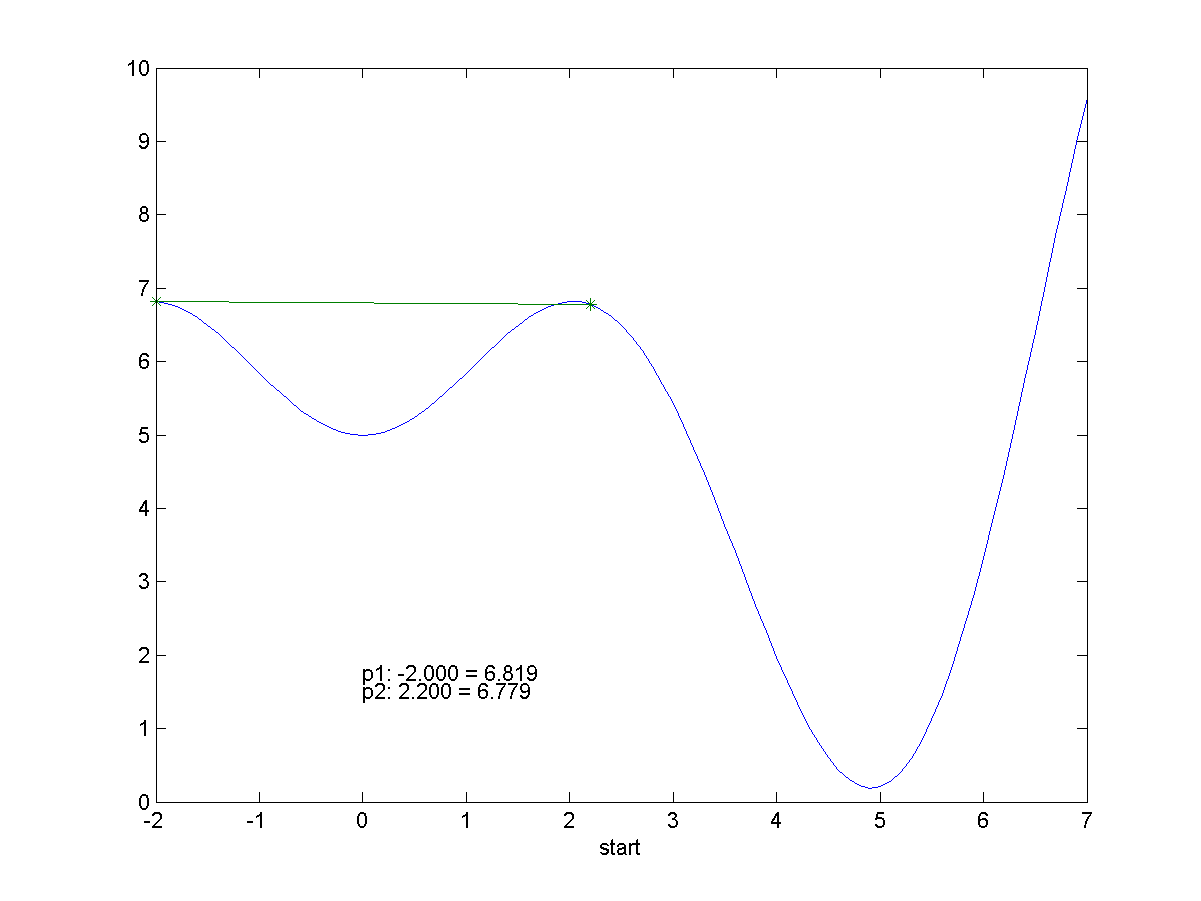
\includegraphics[width=\textwidth]{../bilder/GlobMinima/sinx_x001.png}
\caption{Startsimplex}
\end{subfigure} \begin{subfigure}[b]{0.49\textwidth}
\centering
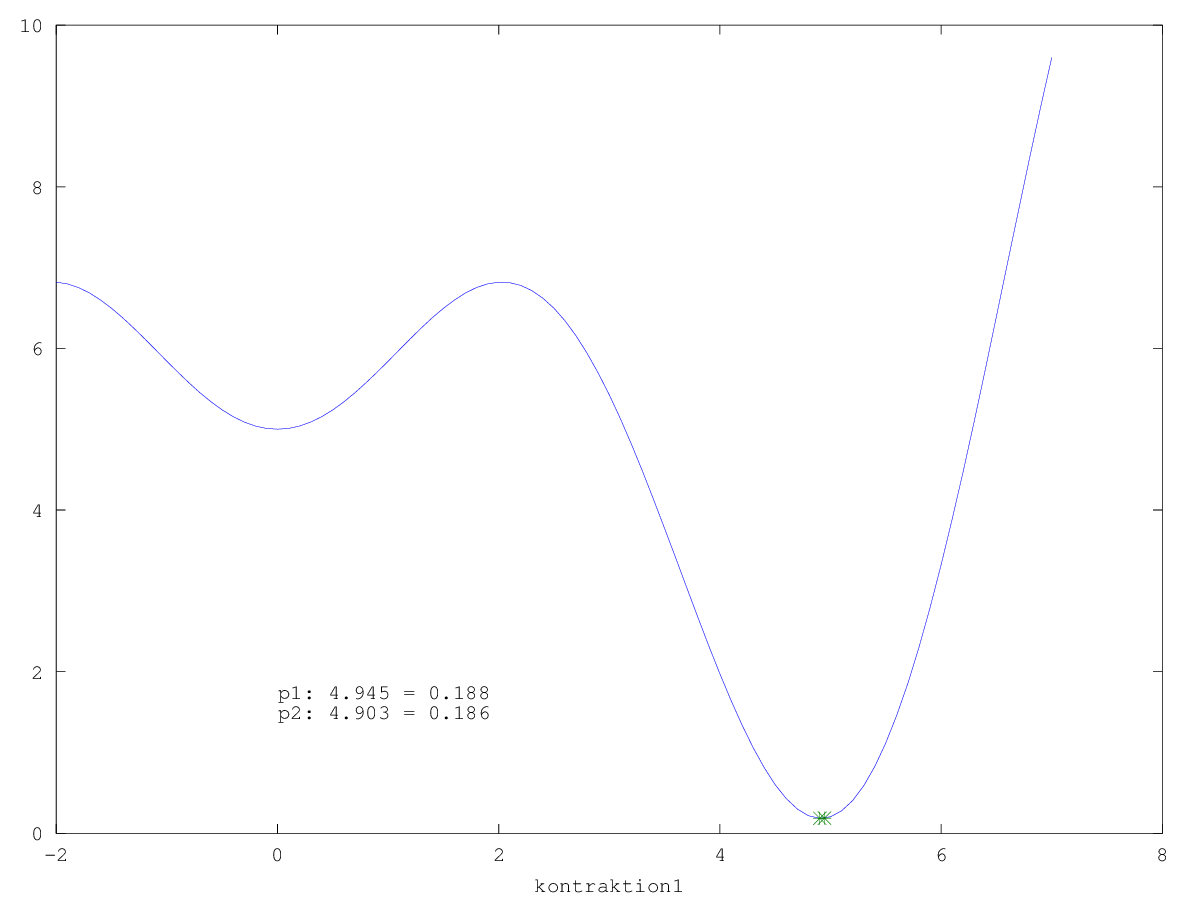
\includegraphics[width=\textwidth]{../bilder/GlobMinima/sinx_x010.png}
\caption{Abbruch mit globalem Minima}
\end{subfigure}
\caption{Globales Minima}
\label{fig:downhillGlobMinima}
\end{figure}


\begin{figure}[htb]
\centering
\begin{subfigure}[b]{0.49\textwidth}
\centering
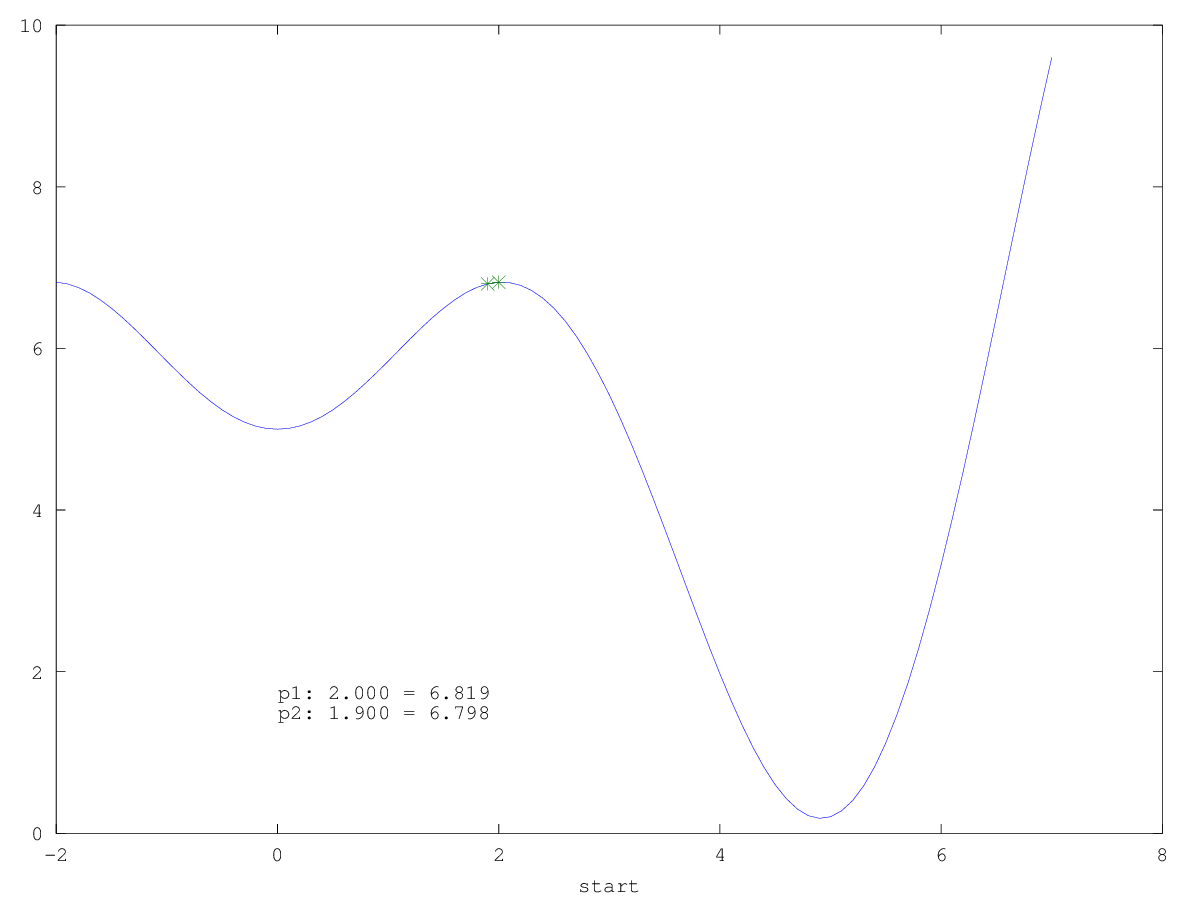
\includegraphics[width=\textwidth]{../bilder/LokMinima/sinx_x001.png}
\caption{Startsimplex}
\end{subfigure} \begin{subfigure}[b]{0.49\textwidth}
\centering
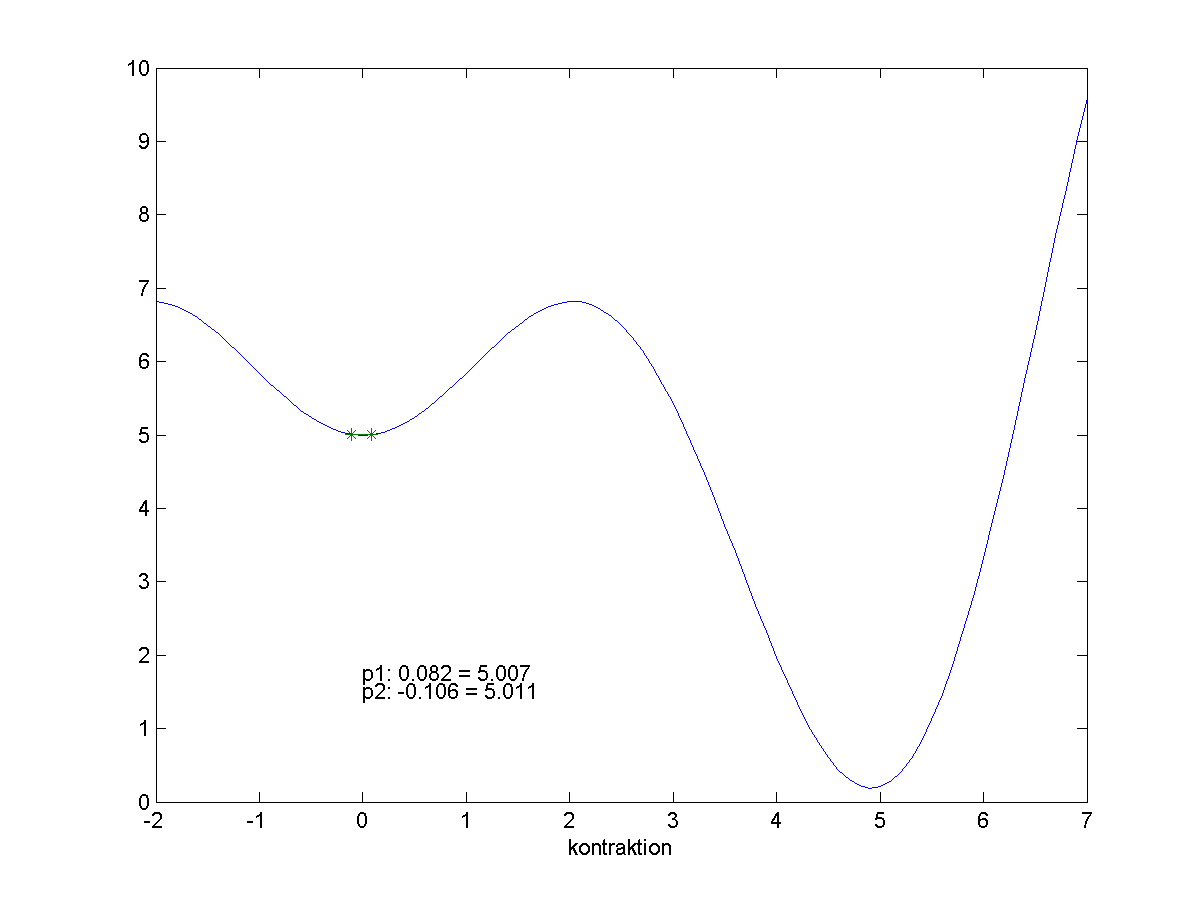
\includegraphics[width=\textwidth]{../bilder/LokMinima/sinx_x010.png}
\caption{Abbruch mit lokalem Minima}
\end{subfigure}

\caption{Lokales Minima}
\label{fig:downhillLokMinima}
\end{figure}

In \figref{fig:downhillGlobMinima} sieht man wie bei gut gew"ahltem Startsimplex der Algorithmus im globalen Minimum konvergiert.
Hingegen in \figref{fig:downhillLokMinima} konvergiert er auf ein lokales Minimum.


\subsubsection{Fr"uhzeitiges Zusammenziehen}
\label{sec:downhillZusammenziehen}
Der Algorithmus kann sich bei schlecht gew"ahltem Startsimplex und oder Parametern fr"uhzeitig zusammenziehen ohne in einem Minimum zu sein.
Das kann verhindert werden indem man das Startsimplex "uber ein gr"osseres Gebiet aufspannt oder den Parameter $\beta$ gr"osser w"ahlt.


\begin{figure}[htb]
\centering
\begin{subfigure}[b]{0.49\textwidth}
\centering
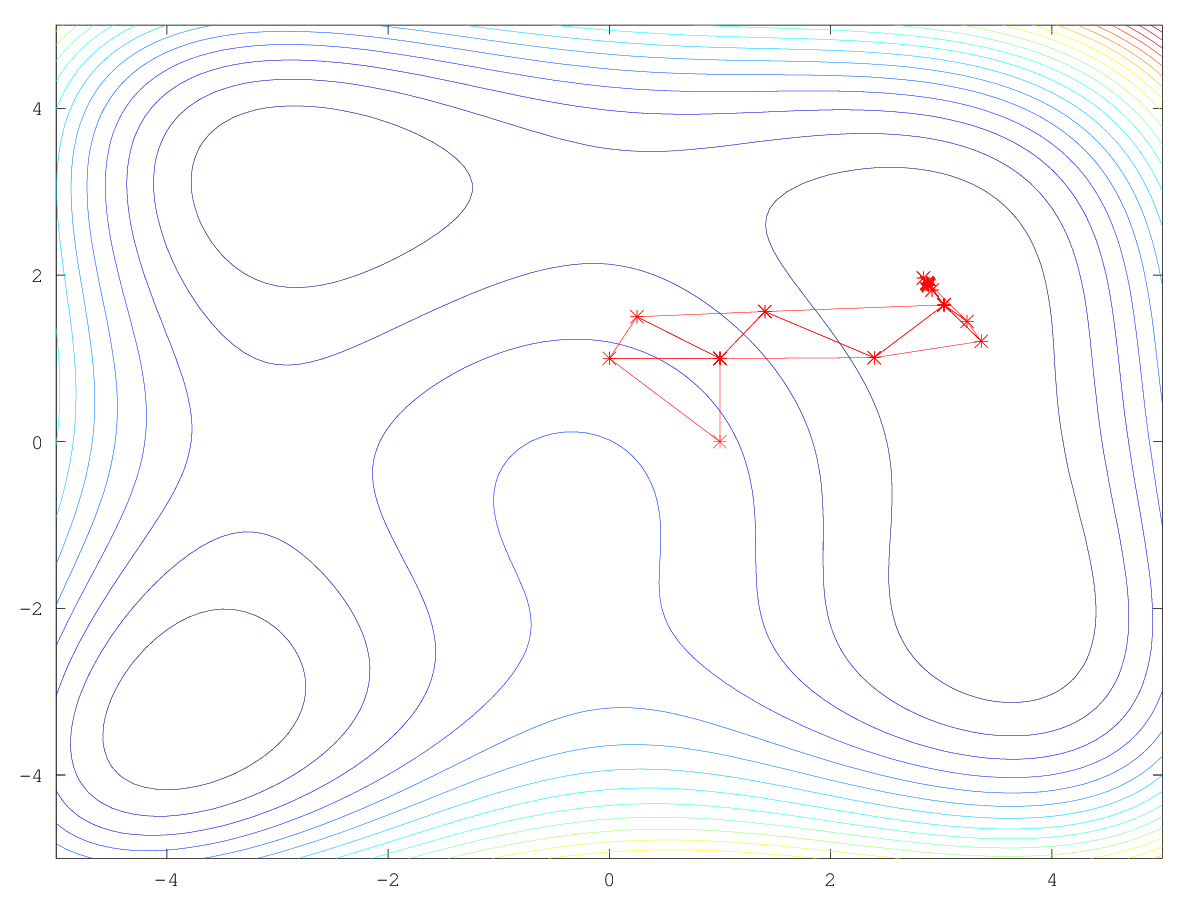
\includegraphics[width=\textwidth]{../bilder/HimmelblauBad/himmelblauall.png}
\caption{Schlecht gew"ahlte Parameter: $z=0.967$}
\end{subfigure} \begin{subfigure}[b]{0.49\textwidth}
\centering
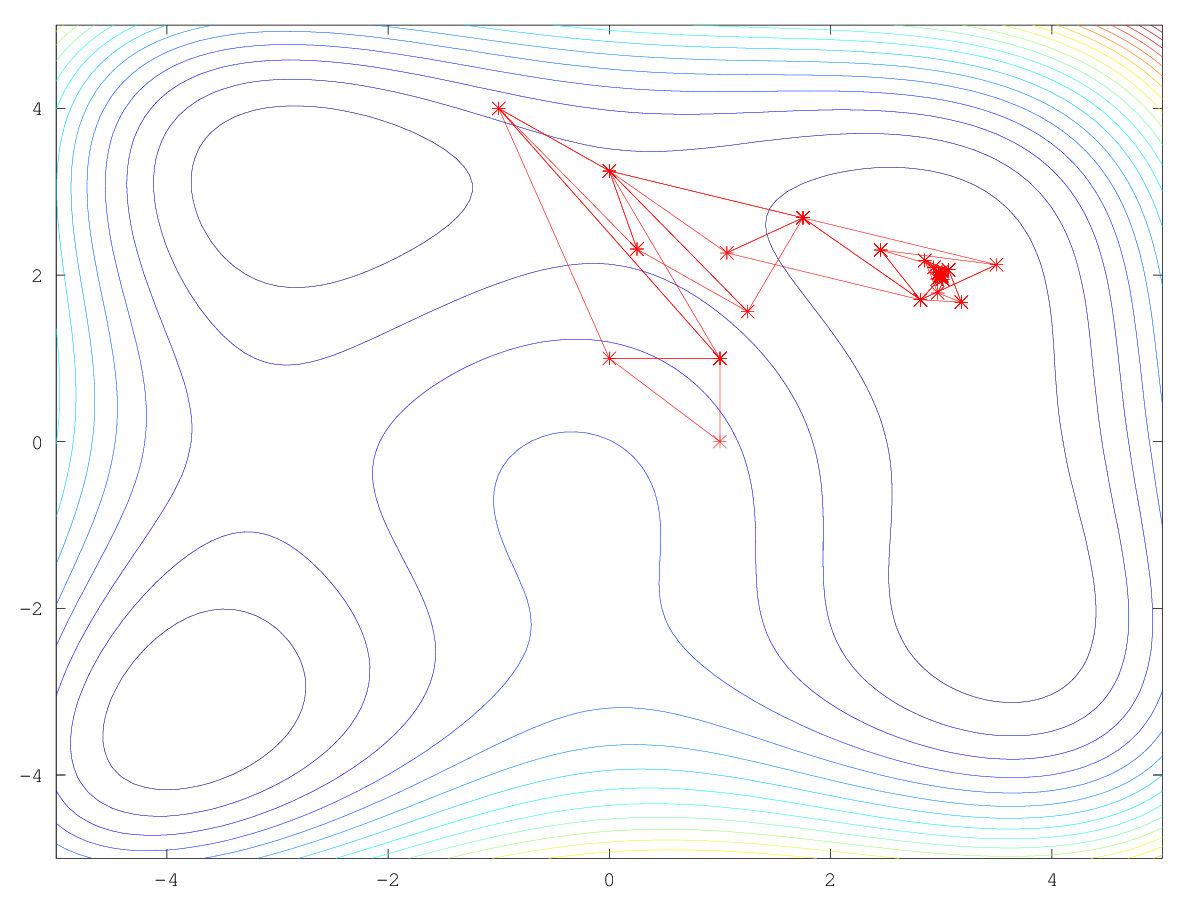
\includegraphics[width=\textwidth]{../bilder/HimmelblauGood/himmelblauall.png}
\caption{Gut gew"ahlte Parameter: $z=0.000$}
\end{subfigure}

\caption{Simplex Verlauf "uber Himmelblau Funktion}
\label{fig:downhillHimmelblau}
\end{figure}

\section{Beispiele}
Auf Grund seines eher einfachen Entscheidungsverfahren ist es nicht sehr aufwendig den Algorithmus in einer entsprechenden Programmiersprache wie C zu implementieren. Eine Schleife mit den richtigen if-else-Abfragen und man hat einen funktionierenden Simplex-Downhill programmiert.\\
Nat"urlich ist der Algorithmus auch in Matlab integriert, man kann ihn mittels der Funktion \textbf{fminsearch} aufrufen. 
Der einfachste Aufruf erfolgt, indem man der Funktion \textbf{fminsearch} die Zielfunktion \textbf{fun} sowie den Startwert \textbf{$x_0$} "ubergibt. Wobei der R"uckgabewert ein neuen x-Wert ist, welcher den Funktionswert $fun(x)$ kleiner werden l"asst. 
\begin{lstlisting}
	x = fminsearch(fun,x0)
\end{lstlisting} 
Will man nun beispielsweise beobachten, wie der Algorithmus das Minima sucht, kann man folgenden Code verwenden: 
\begin{lstlisting}[style=Matlab]
%------------------------------------------------------------
%Initialisierung
%------------------------------------------------------------
xBorder = 10; 
teration = 20; 
x = (-xBorder:0.1:xBorder);				%Dimensionen x und y
y = (-xBorder:0.1:xBorder); 

[xx, yy] = meshgrid(x,y);	%meshgrid f"ur sp"atere Ausgabe
Fun = FUNKTION_SEINER_WAHL(xx,yy); %Berechne gew"unschte Funktionswerte

x_newFun = [4.9,4.9];			%Startwert
z_newFun = 0; 					%Funktionswert
x_Fun = zeros(2,2*teration+1); 	%Vektor f"ur x1,x2
z_Fun = zeros(1,2*teration+1);	%Vektor f"ur Funktionswerte
options = struct('MaxIter',3);	%Einstellungen fminsearch
%------------------------------------------------------------
%Berechnung Simplex-Downhill
%------------------------------------------------------------
for i=1:(2*teration+1)
	[x_newFun z_newFun] = fminsearch(@FUNKTION_SEINER_WAHL,x_newFun,options2);
	x_Fun(1,i) = x_newFun(1,1);
	x_Fun(2,i) = x_newFun(1,2); 
	z_Fun(i)   = z_newFun; 
end
%------------------------------------------------------------
%Ausgabe Resultate
%------------------------------------------------------------
%Darstellung mittels H"ohenlinien
figure; 
contour(xx,yy,Fun,50); 		%Zahl am Ende gibt an, wieviele H"ohenlinien geplottet werden sollen
hold on; 
for i=1:length(x_Fun)		%For-Schleife f"ur Visualisierung
    plot(x_Fun(1,i),x_Fun(2,i),'-*r'); 
    pause(0.5)				%Pause von 0.5 Sekunden
end
hold off; 

%Darstellung in 3D
figure; 
mesh(xx,yy,Fun);
hold on; 
plot3(x_Fun(1,:),x_Fun(2,:),z_Fun(:),'r','linewidth',4); 
hold off; 
grid on; 
\end{lstlisting}
Mittels dem in der Initialisierung definierten Struct kann man der Funktion einige Optionen "ubergeben. 
In diesem Fall wird dem Algorithmus mitgeteilt, wieviele Iterationen er in einem Mal aufrufen durchf"uhren soll. 
Wenn man - wie in unserem Fall - die Werte beobachten will, so sollte diese Zahl m"oglichst klein sein, darf jedoch nicht kleiner als 2 sein. 
Im folgenden wurde der Code auf die Himmelblau-Funktion angewendet: 
\begin{equation}
	f_{hb} = (x_1^2 + x_2 -11)^2 + (x_1+x_2^2-7)^2
\end{equation}
Diese Funktion hat 4 globale Minima: 
\begin{subequations}
	\begin{align}
		f(3,2) &= 0 \\
		f(-2.81,3.13) &= 0\\
		f(-3.78,-3.28) &= 0\\
		f(3.58,-1.85) &= 0
	\end{align}
\end{subequations}
Auf die Funktion wurden zwei Simplex los gelassen, je in gegen"uberliegenden Ecken (9,9) und (-9,-9). Beim roten Simplex ist die Anzahl interner Iterationen von \textbf{fminsearch} auf 2, beim schwarzen Simplex ist die Iteration auf 6 eingestellt.\\
Rein intuitiv ist es klar, dass das schwarze Simplex schneller Richtung Minima konvergiert als das rote Simplex, was in den nachfolgenden Bildern auch zu erkennen ist. \\
Ausserdem sieht man auch deutlich, dass beide Simplexe das ihnen n"achstgelegene Minima ansteuern. 
\begin{figure}[h]
	\centering
	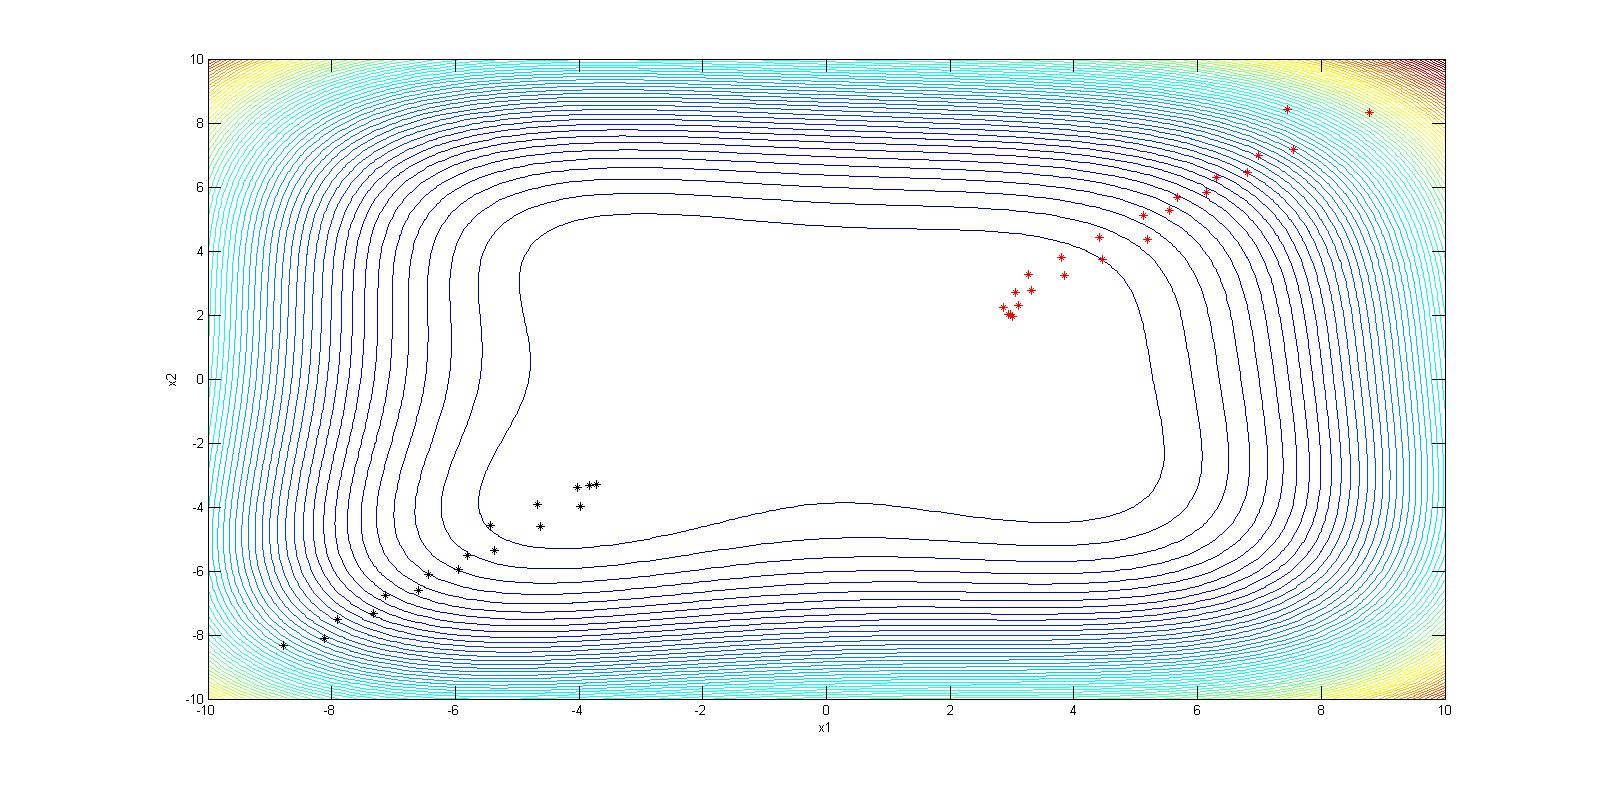
\includegraphics[width=0.8\textwidth]{../bilder/HimmelblauHoehen.jpg}%
  	\caption{Simplexe auf Himmelblau-Funktion}%
	\label{fig:HB1}%
\end{figure}
\newpage
\begin{figure}[h]
	\centering
	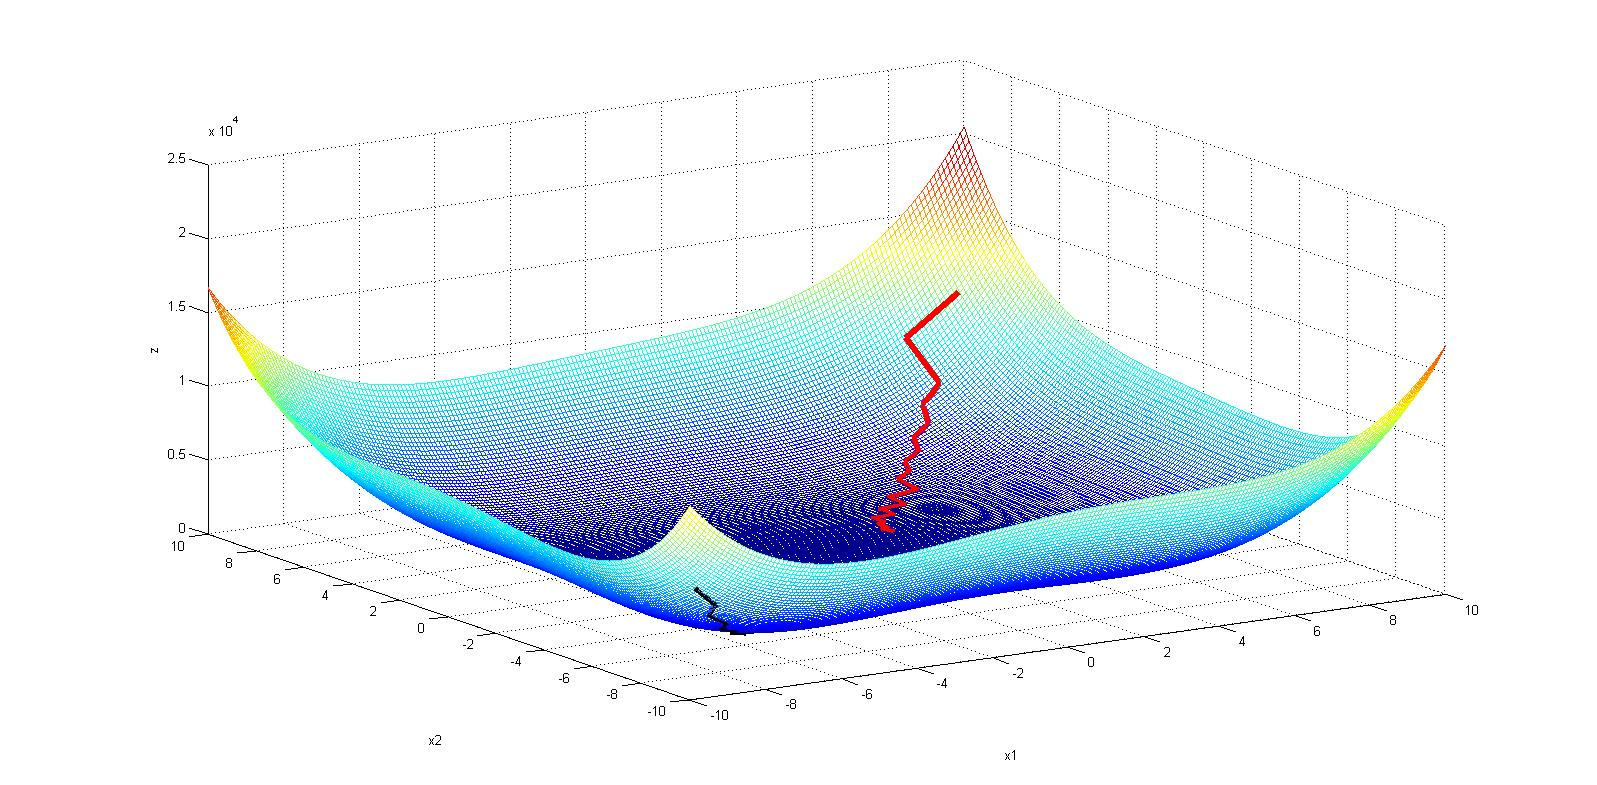
\includegraphics[width=0.8\textwidth]{../bilder/Himmelblau3DRot.jpg}%
  	\caption{Rotes Simplex mit interner Iteration von 3}%
	\label{fig:HB2}%
\end{figure}
\begin{figure}[h]
	\centering
	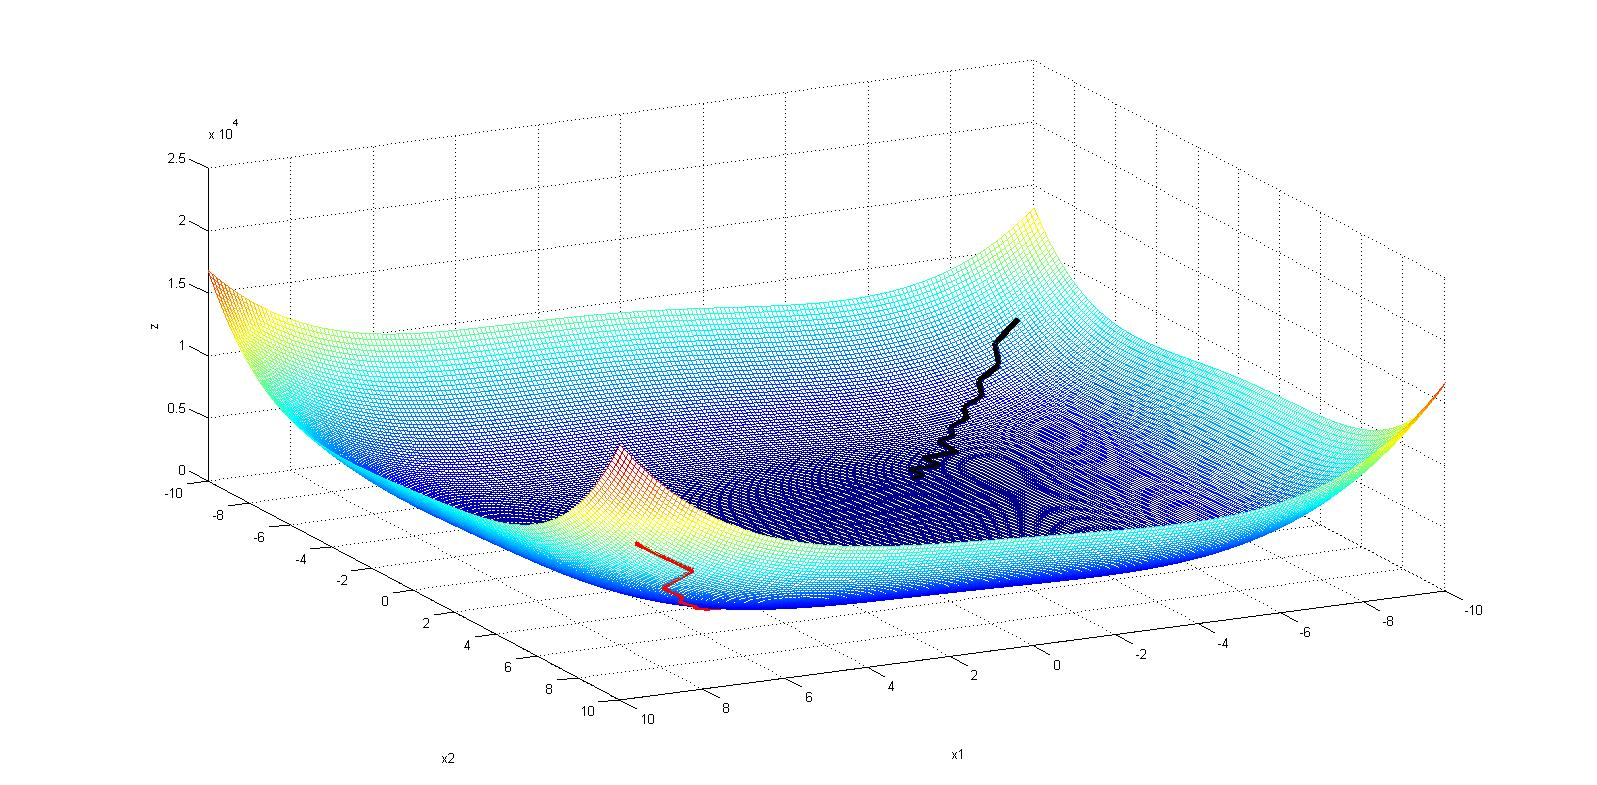
\includegraphics[width=0.8\textwidth]{../bilder/Himmelblau3DSchwarz.jpg}%
  	\caption{Schwarzes Simplex mit interner Iteration von 6}%
	\label{fig:HB3}%
\end{figure}

Beim folgenden Bild sieht man, wie der Algorithmus auf die Quadratfunktion angewendet wird, die interne Iterationszahl von \textbf{fminsearch} ist dabei auf 2 gesetzt und der Algorithmus wird 20 mal durchgef"uhrt.\\
In der Graphik sieht man, dass der Algorithmus eher langsam konvergiert, jedoch von beiden Seiten her dasselbe Resultat erzielt. 
\begin{figure}[h]
	\centering
	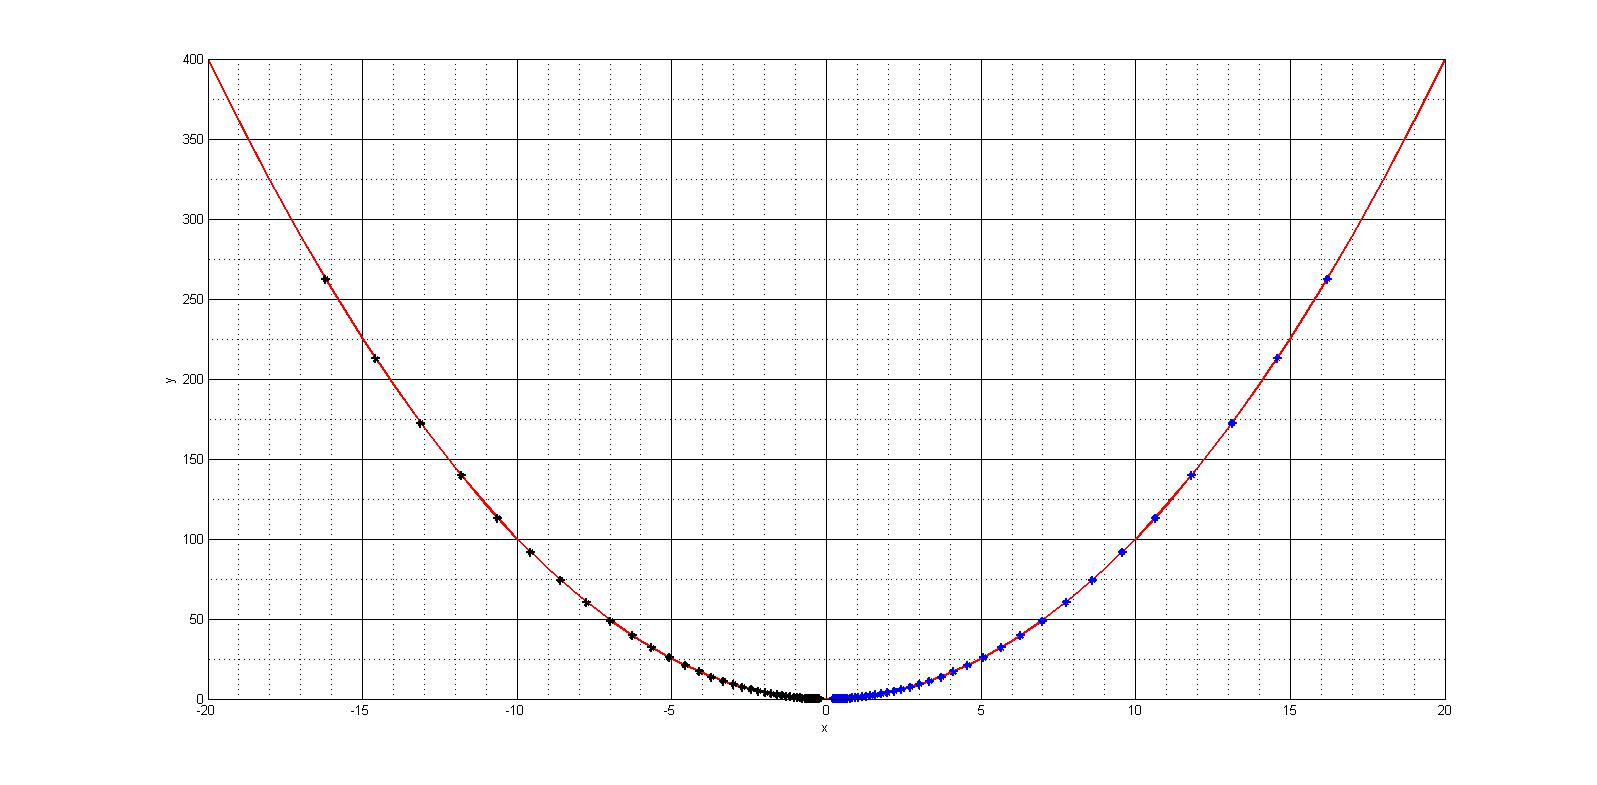
\includegraphics[width=0.8\textwidth]{../bilder/Quadrat.jpg}%
  	\caption{Simplex-Downhill auf Quadratfunktion angewendet}%
	\label{fig:SQ1}%
\end{figure}
\section{Variationen}
Es gibt verschiedenste Variationen des Downhill-Simplex Algorithmus.
Einige verwenden zusätzliche Freiheitsgrade, wie z.B. einen Parameter
$\sigma$, welcher $\beta$ bei Komprimierung ersetzt.

Auch gibt es Erweiterungen welche statistische Auswertung bei verrauschten Zielfunktionen (siehe \figref{fig:downhillRauschen1}) durchführen.
Verrauschte Zielfunktionen treten unter anderem auf wenn man Parameter für ein System optimieren will, welche sich nur durch Messung vergleichen lassen.
Obwohl auch der ''normale`` Downhill-Simplex mehr oder weniger funktioniert (siehe \figref{fig:downhillRauschen2}) ist da viel Potential vorhanden um das Rauschen zu entfernen. Informationen dazu unter \footnote{\url{http://www.informs-sim.org/wsc91papers/1991_0126.pdf}}
\begin{figure}
\centering
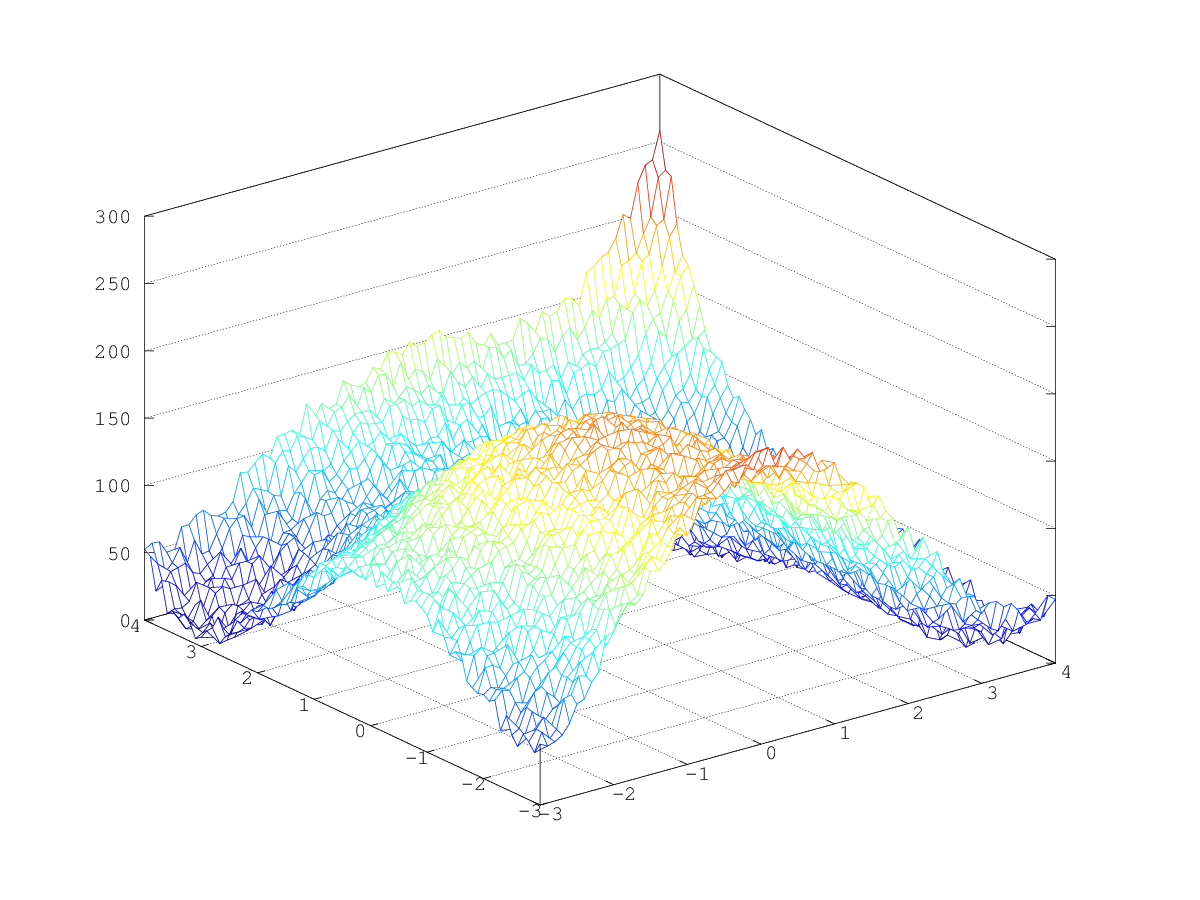
\includegraphics[width=0.8\textwidth]{../bilder/HimmelblauRandom/himmelblauoverview.png}
\caption{Verrauschte Zielfunktion}
\label{fig:downhillRauschen1}
\end{figure}

\begin{figure}
\centering
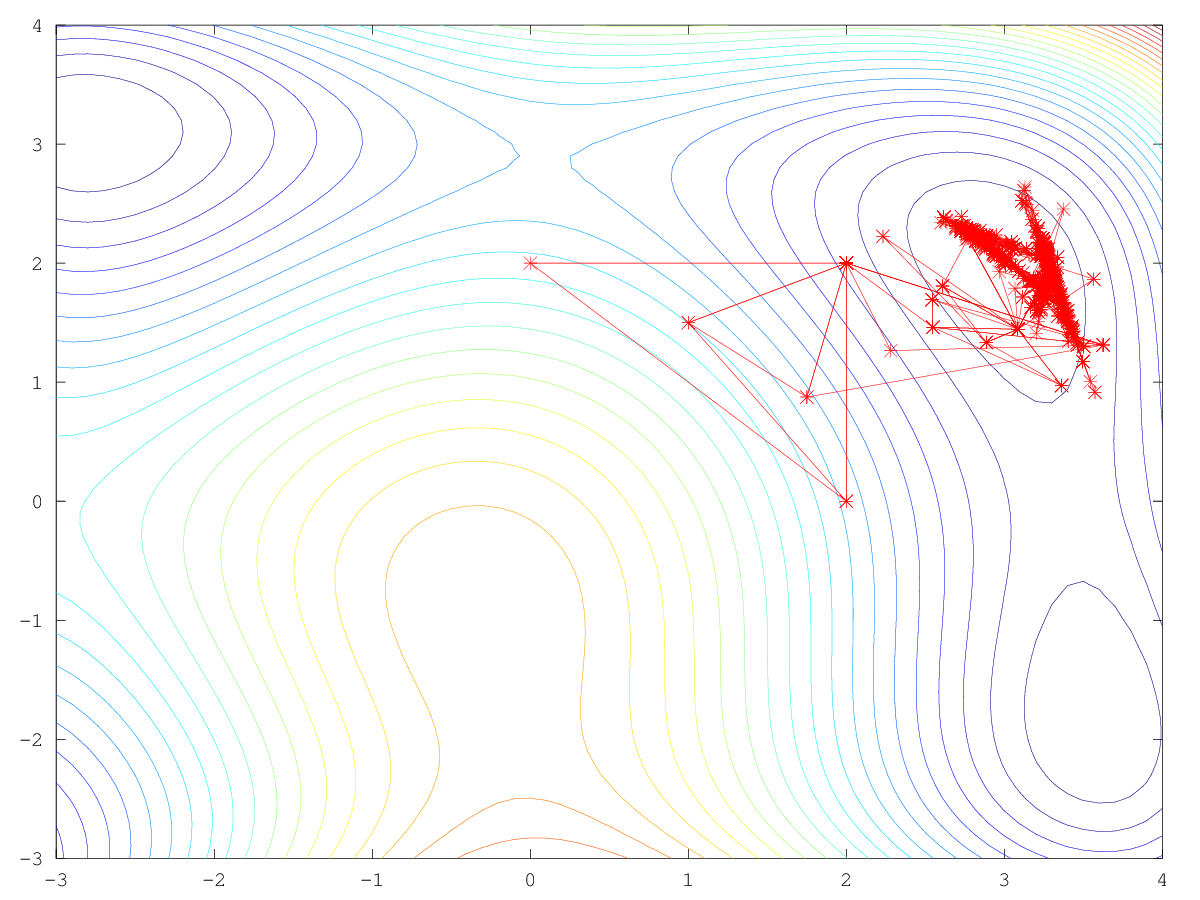
\includegraphics[width=0.8\textwidth]{../bilder/HimmelblauRandom/himmelblauall.png}
\caption{Beispiel Verlauf Simplex mit verrauschter Zielfunktion}
\label{fig:downhillRauschen2}
\end{figure}

\listoffigures
\listoftables

\end{document}
